\documentclass{article}

% if you need to pass options to natbib, use, e.g.:
%     \PassOptionsToPackage{numbers, compress}{natbib}
% before loading neurips_2026

% The authors should use one of these tracks.
% Before accepting by the NeurIPS conference, select one of the options below.
% 0. "default" for submission
\PassOptionsToPackage{numbers,sort&compress}{natbib}
\usepackage[main]{neurips_2026}
% the "default" option is equal to the "main" option, which is used for the Main Track with double-blind reviewing.
% 1. "main" option is used for the Main Track
%  \usepackage[main]{neurips_2026}
% 2. "position" option is used for the Position Paper Track
%  \usepackage[position]{neurips_2026}
% 3. "eandd" option is used for the Evaluations & Datasets Track
 % \usepackage[eandd]{neurips_2026}
 % if you need to opt-in for a single-blind submission in the E&D track:
 %\usepackage[eandd, nonanonymous]{neurips_2026}
% 4. "creativeai" option is used for the Creative AI Track
%  \usepackage[creativeai]{neurips_2026}
% 5. "sglblindworkshop" option is used for the Workshop with single-blind reviewing
 % \usepackage[sglblindworkshop]{neurips_2026}
% 6. "dblblindworkshop" option is used for the Workshop with double-blind reviewing
%  \usepackage[dblblindworkshop]{neurips_2026}

% After being accepted, the authors should add "final" behind the track to compile a camera-ready version.
% 1. Main Track
 % \usepackage[main, final]{neurips_2026}
% 2. Position Paper Track
%  \usepackage[position, final]{neurips_2026}
% 3. Evaluations & Datasets Track
 % \usepackage[eandd, final]{neurips_2026}
% 4. Creative AI Track
%  \usepackage[creativeai, final]{neurips_2026}
% 5. Workshop with single-blind reviewing
%  \usepackage[sglblindworkshop, final]{neurips_2026}
% 6. Workshop with double-blind reviewing
%  \usepackage[dblblindworkshop, final]{neurips_2026}
% Note. For the workshop paper template, both \title{} and \workshoptitle{} are required, with the former indicating the paper title shown in the title and the latter indicating the workshop title displayed in the footnote.
% For workshops (5., 6.), the authors should add the name of the workshop, "\workshoptitle" command is used to set the workshop title.
% \workshoptitle{WORKSHOP TITLE}

% "preprint" option is used for arXiv or other preprint submissions
 % \usepackage[preprint]{neurips_2026}

% to avoid loading the natbib package, add option nonatbib:
%\usepackage[nonatbib]{neurips_2026}

\usepackage[utf8]{inputenc} % allow utf-8 input
\usepackage[T1]{fontenc}    % use 8-bit T1 fonts
\usepackage{hyperref}       % hyperlinks
\usepackage{url}            % simple URL typesetting
\usepackage{booktabs}       % professional-quality tables
\usepackage{amsfonts}       % blackboard math symbols
\usepackage{nicefrac}       % compact symbols for 1/2, etc.
\usepackage{microtype}      % microtypography
\usepackage{xcolor}         % colors
\usepackage{amsmath}
\usepackage{amssymb}
\usepackage{graphicx}
\usepackage{tabularx}
\usepackage{makecell}
\usepackage{listings}
\usepackage{placeins}

% Glossary parameters
\usepackage[acronym, automake]{glossaries}
\usepackage{glossary-mcols}

% Prompt style
\lstdefinestyle{promptstyle}{%
  basicstyle=\ttfamily\footnotesize,%
  breaklines=true,%
  breakatwhitespace=false,%
  columns=fullflexible,%
  keepspaces=true,%
  showstringspaces=false,%
  upquote=true,%
  frame=single,%
  framerule=0.4pt,%
  rulecolor=\color{black!30},%
  backgroundcolor=\color{black!3},%
  xleftmargin=0.5em,%
  xrightmargin=0.5em,%
  aboveskip=0.6em,%
  belowskip=0.6em,%
  literate={--}{{-{}-}}2 {<=}{{<=}}2 {>=}{{>=}}2,%
}
\lstset{style=promptstyle}

\setacronymstyle{long-short}
\makeglossaries
\renewcommand{\glsmcols}{2}
\setglossarystyle{mcolindex}

% Note. For the workshop paper template, both \title{} and \workshoptitle{} are required, with the former indicating the paper title shown in the title and the latter indicating the workshop title displayed in the footnote. 
%\title{ARA: Agentic Reproducibility Assessment Via Structured Reasoning For Scalable Support Of Scientific Peer-Review}
\title{ARA: Agentic Reproducibility Assessment\\For Scalable Support Of Scientific Peer-Review}


% The \author macro works with any number of authors. There are two commands
% used to separate the names and addresses of multiple authors: \And and \AND.
%
% Using \And between authors leaves it to LaTeX to determine where to break the
% lines. Using \AND forces a line break at that point. So, if LaTeX puts 3 of 4
% authors names on the first line, and the last on the second line, try using
% \AND instead of \And before the third author name.


\author{%
  David S.~Hippocampus\thanks{Use footnote for providing further information
    about author (webpage, alternative address)---\emph{not} for acknowledging
    funding agencies.} \\
  Department of Computer Science\\
  Cranberry-Lemon University\\
  Pittsburgh, PA 15213 \\
  \texttt{hippo@cs.cranberry-lemon.edu} \\
  % examples of more authors
  % \And
  % Kevin Riehl \\
  % ETH Zürich, Agentic Systems Lab & Institute for Transport Planning and Systems (IVT) \\
  % Stefano Franscini Platz 5, 8093 Zürich, Switzerland \\
  % \texttt{kriehl@ethz.ch} \\
  % \And
  % Anastasios Kouvelas \\
  % ETH Zürich, Institute for Transport Planning and Systems (IVT) \\
  % Stefano Franscini Platz 5, 8093 Zürich, Switzerland \\
  % \texttt{kouvelas@ethz.ch} \\
  % \And
  % Michail A. Makridis \\
  % ETH Zürich, Institute for Transport Planning and Systems (IVT) \\
  % Stefano Franscini Platz 5, 8093 Zürich, Switzerland \\
  % \texttt{mmakridis@ethz.ch} \\
  % \And
  % Robert Jakob \\
  % ETH Zürich, Agentic Systems Lab \\
  % Weinbergstrasse 56, 8092 Zürich, Switzerland \\
  % \texttt{E-Mail: rjakob@ethz.ch} \\
  % \And
  % Andres L Marin \\
  % Affiliation \\
  % Address \\
  % \texttt{andreslaverdemarin@gmail.com} \\
  % \And
  % Nikiforos Zacharof \\
  % Affiliation \\
  % Address \\
  % \texttt{zacharof@auth.gr} \\
  % \And
  % Georgios Fontaras \\
  % Affiliation \\
  % Address \\
  % \texttt{georgios.fontaras@ftco.eu} \\
}


\begin{document}


\maketitle




%%%%%%%%%%%%%%%%%%%%%%%%%%%%%%%%%%%%%%%%%%%%%%%%%%%%
\begin{abstract}
% Scientific peer review increasingly struggles to assess reproducibility at the scale and complexity of modern research output. 
% While reproducibility is central to scientific reliability, evaluating it requires reconstructing experimental dependencies, methodological choices, data flows, and result-generating procedures -- efforts that goes beyond what human reviewers can afford.
% Agentic Reproducibility Assessment (ARA) is a domain-agnostic framework that formalizes reproducibility assessment as a structured reasoning task over scientific documents. 
% Given a paper, ARA uses LLM-based agents to extract a directed workflow graph linking sources, methods, experiments, and outputs, and then evaluates the reconstructability of this graph through complementary structural and content-based scores. 
% %Unlike checklist-based approaches, ARA assesses whether reported claims can be traced through coherent methodological pathways and whether individual workflow components contain sufficient information for independent reconstruction. 
% Computational experiments using 213 articles from ReScience C -- the largest cross-domain benchmark of human-validated computational reproducibility studies considered to date -- demonstrate the consistency of the workflow reconstruction and assessment across LLM-models, temperatures, and corpus-level analyses.
% The results demonstrate ARA's potential to complement human assessments at scale, offering a practical foundation for next-generation peer review. 
% %Across LLM-model, temperature, and corpus-level analyses, ARA produces stable reproducibility profiles and identifies content-level underspecification as the primary bottleneck, despite generally strong workflow reconstruction. 
% %Our results suggest that agentic systems can provide scalable, interpretable support for reproducibility auditing and offer a practical foundation for next-generation peer-review infrastructure.
%
Scientific peer review increasingly struggles to assess reproducibility at the scale and complexity of modern research output.
Evaluating reproducibility requires reconstructing experimental dependencies, methodological choices, data flows, and result-generating procedures, which often exceeds what human reviewers can provide.
Agentic Reproducibility Assessment (ARA) formalizes reproducibility assessment as a structured reasoning task over scientific documents.
Given a paper, ARA extracts a directed workflow graph linking sources, methods, experiments, and outputs, then evaluates its reconstructability using structural and content-based scores for reproducibility assessments.
Experiments on 213 ReScience C articles -- the largest cross-domain benchmark of human-validated computational reproducibility studies considered to date --demonstrate ARA's generalizability and consistent workflow reconstruction and assessment across LLMs, model temperatures, and scientific domains.
These results highlight ARA's potential to complement human review at scale and support next-generation peer review.
\end{abstract}




%%%%%%%%%%%%%%%%%%%%%%%%%%%%%%%%%%%%%%%%%%%%%%%%%%%%
\section{Introduction}

% Paragraph 01: Explosion of scientific output grows exponentially → evaluation reliability is becoming increasingly harder, but traditional quality control (peer-review) doesnt scale with that growth, leading to significant quality issues in science
Scientific publication output has grown exponentially across disciplines over the past decades, driven by expanding global research communities, increasing specialization of venues, and strong incentive structures tied to publication productivity~\citep{parchomovsky2000publish,szalay2006science}. 
More recently, the emergence of large language models (LLMs) as writing assistants has further accelerated manuscript production, raising concerns about declining signal-to-noise ratios in the scientific literature~\citep{mosca2023distinguishing,cheng2024have}. 
While increased output reflects healthy research activity, it also places substantial pressure on traditional mechanisms of quality assurance such as peer review (the backbone of modern science), that was designed for slower and smaller publishing ecosystems~\citep{zhou2024llm}. 
Today, reviewers face growing workloads, limited time, and heterogeneous evaluation standards, making it increasingly difficult to maintain consistent quality assessment across submissions~\citep{ellison2011peer}. 
As a result, scalable support mechanisms for evaluating the quality and reliability of scientific claims are becoming an urgent requirement~\citep{wei2025ai}.

% Paragraph 02: reproducibilty is the most important quality aspect of scientific literature, and we can already observe a reproducibility crises in many fields, especially reviewing reproduicbility of a study requires efforts that go beyond what human reviewers that are not even remunerated can offer
Among the various dimensions of scientific quality, reproducibility occupies a central role as a necessary condition for validating scientific contributions~\citep{popperDE,popperEN}. 
However, large-scale meta-analyses across multiple disciplines including psychology~\citep{anvari2018replicability}, medicine and biomedical sciences~\citep{errington2014open,stupple2019reproducibility,miyakawa2020no}, social and behavioral sciences~\citep{fivsar2024reproducibility,tyner2026investigating}, and computer science~\citep{hutson2018artificial,riehl2025revisiting} have documented a substantial reproducibility crisis~\citep{baker2016reproducibility,fanelli2018science}.
Many published studies omit essential implementation details such as parameter settings, preprocessing steps, or access to datasets and source code, limiting the ability of researchers to independently verify reported findings and to assess the generalizability of the resulting knowledge~\citep{stark2018before}.
Importantly, assessing reproducibility is not equivalent to evaluating narrative clarity or novelty; it requires reconstructing procedural dependencies and experimental pipelines, often across multiple methodological layers. 
Such efforts exceed what volunteer peer reviewers can realistically provide during standard evaluation cycles. 
Consequently, reproducibility assessments remain underrepresented in standard peer-review evaluation workflows, and difficult to scale relative to the volume of published research~\citep{national2019reproducibility}.
%These challenges are particularly pronounced in machine learning research, where complex experimental pipelines and implicit implementation choices frequently hinder independent verification.

% Paragraph 03: now opportunity, agentic AI and LLMs as scientific evaluators, emerging technology, because they are scalable technology, proof to work well with large texts and reasoning tasks
Recent advances in LLMs and agentic reasoning systems suggest a new opportunity to address this gap. 
Modern agent pipelines are capable of operating over long technical documents, extracting structured procedural information, identifying dependencies between experimental components, and performing multi-step reasoning tasks across heterogeneous textual evidence~\citep{acharya2025agentic}. 
Unlike manual review processes, these systems scale naturally with corpus size and can be deployed consistently across large collections of scientific articles. 
This creates the possibility of operationalizing reproducibility assessment itself as a structured reasoning problem that can be partially automated~\citep{li2025generation}.
Rather than replacing human replication efforts, agentic systems may provide scalable diagnostic support for identifying missing reporting elements, incomplete workflows, and reproducibility bottlenecks in scientific publications.
This suggests that reproducibility assessment may be tractable as a document-level reasoning task rather than requiring full experimental replication~\citep{jin2024agentreview,thakkar2025can}.
% Previous work and its limitations
Previous work has demonstrated the potential of agentic systems for peer-review~\citep{liang2024can,hossain2025llms,zhuang2025large}, to assess reproducibility ~\citep{hu2025repro,nguyen2026replicatorbench}, or even to reproduce papers~\citep{kim2025reproduction,seo2025paper2code}. However, these preliminary approaches are limited to specific domains, rely on simple techniques such as document-parsing and checklist-based approaches rather than reasoning the structure of the paper, and therefore lack generalizability. 

% Paragraph 04: what this paper proposes, "Rather than automating replication itself, we study whether agentic systems can approximate reproducibility assessment as a structured reasoning task."
In this work, we investigate whether and how reproducibility assessment can be formalized as a structured reasoning task executable by agentic AI systems. 
%Rather than automating replication itself, we study whether agentic systems can approximate reproducibility assessment as a structured reasoning process. 
To this end, we introduce \texttt{Agentic Reproducibility Assessment (ARA)}, a pipeline that uses LLM agents to analyze scientific papers and construct interpretable graph representations of their methodological structure and results. 
In the first step, \texttt{ARA} converts scientific works into workflow graphs, and identifies required reproduction components.
In the second step, it projects this workflow graph to reproducibility assessments (scoring) across multiple reproducibility dimensions.
%, including availability, transparency, parameter specification, procedural clarity, and experimental design completeness. 
%Instead of producing binary judgments, the framework generates structured reproducibility profiles that characterize the extent to which studies provide sufficient information for independent verification.
%Unlike prior checklist-based or heuristic reproducibility scoring approaches~\citep{meyerholz2018principles,riehl2025revisiting}, ARA models reproducibility as a workflow reconstruction problem and evaluates reporting completeness through structured dependency extraction across methodological components.
% Paragraph 05: Empirical vlaidation using Rescience C
We evaluate the proposed framework using 213 scientific publications (largest dataset to date) from \textit{ReScience C} -- a journal dedicated to computational reproducibility studies across a multitude of scientific disciplines~\citep{rougier2018rescience}. 
Papers in this venue provide structured documentation of human replication attempts and therefore constitute a uniquely suitable benchmark dataset for assessing automated reproducibility diagnostics versus human assessments.
Using this dataset as a benchmark, we compare agent-generated reproducibility assessments with verified reproduction workflows and reporting structures.
The experiments are complemented by consistency checks across different LLMs, temperatures, and further benchmark datasets.
Our results demonstrate the domain-agnostic capabilities of \texttt{ARA}, and that the proposed agentic reproducibility analysis captures meaningful signals aligned with real-world reproducibility requirements beyond mere checklist-based document parsing. % and successfully identifies key components necessary for reconstructing experimental pipelines. 
%These findings provide empirical evidence that reproducibility assessment can be approximated through structured document-level reasoning performed by LLM-based agent systems.


\begin{figure}[!hb]
    \centering
    
\includegraphics[width=\linewidth]{figures/Figure_ARA_Pipeline.pdf}
    \caption{
\textbf{Agentic Reproducibility Assessment Pipeline (\textit{ARA}).}
First, a given scientific paper (resp. document) $D$ is transformed into a directed workflow graph $G$, comprising four types of nodes (sources, methods, experiments, sinks). 
Second, the workflow graph's reconstructability is projected on micro-level assessments of reproducibility (node-by-node) $r(\cdot)$.
Third, the micro-level assessments are aggregated to reproducibility scores $R_k$ and $R$.
    }\label{fig:ara_pipeline}
\end{figure}


% Paragraph 06: Why this metters and summray of significance
%The proposed approach contributes to emerging efforts at the intersection of artificial intelligence and infrastructure for scientific reliability assessment by introducing a scalable framework for automated reproducibility auditing. 
%More broadly, it demonstrates a new role for agentic AI systems as evaluators of methodological completeness rather than generators of scientific text or code. 
%This capability is particularly relevant for machine learning research, where reproducibility challenges remain persistent despite increasing awareness and the introduction of artifact evaluation protocols. 
%By formulating reproducibility assessment as an agent-executable reasoning task and validating the approach on verified replication literature, our work provides a foundation for integrating agentic evaluation pipelines into future peer-review support systems and large-scale meta-scientific monitoring frameworks. 
%Together, these results suggest that agentic systems can become an important component of next-generation scientific reliability infrastructure.


%\textcolor{red}{Promote not only we develop tool but also labelled reproducibility dataset, Justify why ReScience C: because it is cross-domain, and it is bigger than existing, and also publically available reproduction reports, and }

%\textcolor{red}{In our methods / results / discussion, we could not only show that we can do an assessment and it comes close to human reproduction assessments on ReScience C, but alos highlight limiations or challenges, such as high runtimes, and other questions like: •	Critical questions we could also ask: o	Why do AI agents fail to reproduce and analyze results? o	Why do AI agents fail to recognize inconsistencies?}

%\textcolor{red}{MustRead for all Coauthors: "REPRO-BENCH: Can Agentic AI Systems Assess the Reproducibility of Social Science Research?" They come closest to us, but still we are better than them (see literature review)}

%\textcolor{red}{Emphasize we go beyond mere checklist based assessment automation, we are capturing multi-dimensionality of reproducibility assessment much better, we are cross-domain, we have super big dataset we evaluate on (compared to all previous efforts), how to phrase our approach? structure reasoning or something}

%%%%%%%%%%%%%%%%%%%%%%%%%%%%%%%%%%%%%%%%%%%%%%%%%%%%
\section{Related Work}

Prior work on reproducibility assessment spans checklist-based evaluation frameworks, automated reconstruction of experimental workflows from scientific papers, and recent efforts to apply LLM agents to peer review and replication support. 
These developments suggest that scientific reliability assessment can increasingly be approached as a structured document-level reasoning task. 
However, existing approaches remain largely domain-specific, depend on predefined reporting metrics, or assume access to replication packages beyond the publication itself. 
In the following, we review related work across these directions and position \texttt{ARA} as a domain-agnostic workflow reconstruction framework for scalable reproducibility assessment directly from scientific papers.

% somehow mention how central reproducibility is, one of most pressing issues (2026_Kubota)
% talk about that LLMs and generative models have transformed the way we work, becoming part of scientific workflow not only on generation side but also on the consuming side;
% therefore the performance of the llms better and better and might help address review process problem

% Paragraph 01: reproducibility assessment
\paragraph{Reproducibility Assessment.}
Reproducibility is a foundational principle of modern scientific practice because it enables independent verification of empirical claims~\citep{riehl2025revisiting} and supports the falsification criterion central to Popperian critical rationalism~\citep{popperDE,popperEN}. 
Prior work conceptualizes reproducibility as a multi-dimensional construct encompassing the availability of supplementary materials and digital research artifacts~\citep{riehl2025revisiting,stagge2019assessing}, the reliability and repeatability of methodological procedures~\citep{downing2004reliability,bazzocchi2011accuracy,crowley2016critical,bunting2019practical}, transparency in statistical reporting~\citep{hung2020statistical,held2024assessment}, and the use of standardized benchmarks and harmonized experimental protocols~\citep{crowley2016critical,arroyo2022systematic}. 
Additional work emphasizes systematic reporting of data quality and experimental assumptions, as well as the development of quantitative reproducibility indicators beyond qualitative reporting assessments~\citep{crowley2016critical}. 
Empirical meta-research further documents persistent barriers to reproducibility assessment, including missing descriptive statistics, unavailable datasets, insufficient methodological detail, and limited author responsiveness to clarification requests~\cite{errington2014open}. 
Despite these advances, most reproducibility assessment frameworks remain domain-specific and rely on checklist-based criteria that capture only limited aspects of methodological completeness, limiting their generalizability across disciplines and their scalability to the rapidly growing volume of scientific publications.
% •	[2025_Riehl] riehl reproducibility (transparency of repositories)
% •	[2018_Meyerholz] https://www.sciencedirect.com/science/article/pii/S0023683722010194
% principles (Checklist based) meyerholz2018principles
% •	[2025_Shyr] https://www.medrxiv.org/content/10.1101/2025.08.06.25333170v3
% A statistical framework for evaluating the repeatability and reproducibility of large language models
% •	[2004_Downing] https://asmepublications.onlinelibrary.wiley.com/doi/full/10.1111/j.1365-2929.2004.01932.x
% Reliability: on the reproducibility of assessment data
% •	[2011_Bazzocchi] https://www.sciencedirect.com/science/article/pii/S1076633211002406
% Accuracy, Reproducibility and Repeatability of Ultrasonography in the Assessment of Abdominal Adiposity
% •	[2023_Fisar]https://pubsonline.informs.org/doi/full/10.1287/mnsc.2023.03556
% Reproducibility in Management Science
% •	[2018_Stagge] https://www.nature.com/articles/sdata201930
% Assessing data availability and research reproducibility in hydrology and water resources
% •	[2020_Hung] https://www.jstor.org/stable/27119678
% STATISTICAL METHODS FOR REPLICABILITY ASSESSMENT 
% •	[2021_errington] https://elifesciences.org/articles/67995
% Reproducibility in Cancer Biology: Challenges for assessing replicability in preclinical cancer biology
% •	[2025_AnkelPeters] https://academic.oup.com/qopen/article/5/3/qoaf004/8090197?guestAccessKey=
% A protocol for structured robustness reproductions and replicability assessments Open Access 
% •	[2021_Pearson] https://psycnet.apa.org/buy/2021-78188-001
% Examining replicability in addictions research: How to assess and ways forward.
% •	[2022_Arroyo] https://journals.plos.org/plosbiology/article?id=10.1371/journal.pbio.3001886
% Systematic assessment of the replicability and generalizability of preclinical findings: Impact of protocol harmonization across laboratory sites
% •	[2024_Brodeur] https://www.jstor.org/stable/pdf/resrep58994.pdf?acceptTC=true&coverpage=false&addFooter=false
% Mass Reproducibility and Replicability: A New Hope
% •	[2024_Held] https://royalsocietypublishing.org/rsos/article/11/8/240149/92746
% The assessment of replicability using the sum of p-values Open Access 
% •	[2019_Bunting] https://www.sciencedirect.com/science/article/pii/S0894731719309460
% A Practical Guide to Assess the Reproducibility of Echocardiographic Measurements
% •	[2016_Crowlye]¨https://www.sciencedirect.com/science/article/pii/S0894731716303972
% Critical Review of Current Approaches for Echocardiographic Reproducibility and Reliability Assessment in Clinical Research
 
% Paragraph 02: agentic ai & llms for replication
\paragraph{Agentic \& LLM-assisted Paper Reproduction.}
Recent advances in LLMs and agentic systems have enabled automated pipelines that translate scientific papers into executable computational workflows, particularly in computer science~\citep{seo2025paper2code,li2025deepcode}, astrophysics~\citep{ye2025replicationbench}, machine learning~\citep{starace2025paperbench}, and quantitative science~\citep{kubota2026llm}, where experiments rely on standardized datasets, statistical models, and software-based implementations~\citep{kubota2026llm}. 
A growing line of work studies document-to-codebase synthesis~\citep{li2025deepcode}, reconstructing repository-level implementations from textual method descriptions through hierarchical information-flow optimization~\citep{li2025deepcode}. 
Related systems such as \textit{PaperCoder} (\textit{Paper2Code})~\citep{seo2025paper2code} further demonstrate that agent pipelines can plan architectures, identify file dependencies, and generate modular implementations from scientific documents. 
Benchmarks including \textit{AutoExperiment}~\citep{kim2025reproduction}, \textit{ReplicationBench}~\citep{ye2025replicationbench}, and \textit{PaperBench}~\citep{starace2025paperbench} evaluate agents’ ability to synthesize experimental code and reproduce reported results. 
Recent work further shows that LLM-based systems can replicate statistical analyses from quantitative social science papers and detect inconsistencies in reported results, supporting their integration into extended scientific workflows~\citep{kubota2026llm,kubota2026llm2,ye2025replicationbench}. 
In contrast to these preliminary, domain-specific approaches, which aim to reconstruct or execute experiments directly, \texttt{ARA} models reproducibility assessment as a structured reasoning task that evaluates methodological dependency completeness without requiring full experimental replication.
% agentic ai for replicating / reproducing papers
% •	Paper2Code https://arxiv.org/abs/2504.17192 
% •	DeepCode https://github.com/HKUDS/DeepCode
% •	https://www.linkedin.com/posts/andrew-hall-40a88444_heres-proof-that-claude-code-can-now-write-activity-7413610180048818177-Fqpk/?utm_source=share&utm_medium=member_android&rcm=ACoAACVnCNwBuCe3TXeYro10prq_QCeCU7bFREg
% •	https://www.youtube.com/watch?v=MQZYpLkzsbw
% •	Reproducibility in the Control of Autonomous Mobility-on-Demand Systems has is recently accepted on T-RO: https://arxiv.org/pdf/2506.07345
% •   https://arxiv.org/abs/2511.04824
% Agentic Refactoring: An Empirical Study of AI Coding Agents
% •   https://arxiv.org/abs/2506.19724
% From Reproduction to Replication: Evaluating Research Agents with Progressive Code Masking
% •   https://arxiv.org/abs/2602.18453
% LLM-Assisted Replication for Quantitative Social Science
% •   https://osf.io/download/69b438a1e600d95c35dc7447/
% LLM-Assisted Replication as Scientific Infrastructure
% •   https://www.science.org/doi/full/10.1126/science.aaf0918
% Evaluating replicability of laboratory experiments in economics
% •   https://arxiv.org/abs/2510.24591
% ReplicationBench: Can AI Agents Replicate Astrophysics Research Papers?

% Paragraph 03: agentic ai for peer review
\paragraph{Agentic \& LLM-assisted Scholarly Peer Review.}
Recent work explores the use of large language models as assistants in scholarly peer review to address growing submission volumes and reviewer workload. 
Empirical studies show that LLM-generated comments substantially overlap with human feedback and are often perceived as similarly helpful by authors, supporting their feasibility for early-stage manuscript evaluation~\citep{liang2024can}. 
Automated reviewing systems have further been proposed for rapid quality screening, meta-review synthesis, and editorial decision support at scale~\citep{tyser2024ai,hossain2025llms}. 
Alternative paradigms evaluate manuscripts through pairwise comparison with existing literature rather than absolute scoring, improving impact identification but introducing risks of topical and institutional bias~\citep{zhang2025replication}. 
At the same time, technical evaluations highlight reliability limitations on longer manuscripts and the need for human oversight~\citep{zhou2024llm}. 
Survey evidence indicates that LLM-assisted reviewing is already widespread, with approximately 19\% of reviewers reporting usage in 2025 and more than 50\% in 2026, raising concerns about transparency and the social contract of peer review~\citep{naddaf2025ai,naddaf2026more}. 
More broadly, increasing reliance on LLM-mediated reviewing may introduce feedback loops in which scientific writing and evaluation co-evolve with model-generated outputs, raising governance challenges for AI-assisted scholarly communication~\citep{zhuang2025large}.
% agentic ai for peer review
% •   https://arxiv.org/abs/2506.11343
% From Replication to Redesign: Exploring Pairwise Comparisons for LLM-Based Peer Review
% •   https://dl.acm.org/doi/abs/10.1145/3701716.3717754
% Towards Agentic AI for Science: Hypothesis Generation, Comprehension, Quantification, and Validation
% References from 2026_Kubota: peer review (Liang et al., 2024; Tyser et al., 2024; Zhou et al., 2024; Zhuang et al., 2025; Hossain et al., 2025; Naddaf, 2025

% Paragraph 04: agentic ai for reproducibility assessment
\paragraph{Agentic \& LLM-assisted Reproducibility Assessment.}

Recent work explores the use of LLMs for automated reproducibility assessment, typically through checklist-based scoring frameworks or domain-specific evaluation pipelines. 
For example, \textit{Reproscreener} evaluates computational reproducibility signals in machine learning preprints using structured reporting metrics derived from publication standards~\citep{bhaskar2024reproscreener}, while \textit{Paper-snitch}~\citep{santoli2024} and \textit{RECAP}~\citep{da2026assessing} automate artifact availability and checklist-style transparency screening in specialized conference corpora. 
Similarly, \textit{Auto-METRICS}~\citep{de2025auto} demonstrates that LLMs can assist methodological quality assessment in radiomics research using standardized domain-specific scoring protocols. 
More recent agent-based benchmarks such as \textit{ReplicatorBench}~\citep{nguyen2026replicatorbench} evaluate end-to-end replication workflows across stages of experimental reconstruction and interpretation, but remain restricted to social and behavioral science settings. 
The closest related work, \textit{REPRO-BENCH} and \textit{REPRO-AGENT}~\citep{hu2025repro}, provides early evidence that agentic systems can assess the reproducibility of social science papers when reproduction packages are available, although their evaluation setting depends on access to code and data and follows predefined scoring schemes derived from existing reproducibility indices. 
In contrast, the proposed framework \texttt{ARA} models reproducibility assessment as a workflow reconstruction problem directly from publications' texts, enabling domain-agnostic reproducibility assessments across substantially larger and more heterogeneous corpora of scientific studies.
% Competitors / Value Proposition / How we are different from them (above them)
% •   https://aclanthology.org/2025.findings-acl.1210/
% REPRO-Bench: Can Agentic AI Systems Assess the Reproducibility of Social Science Research?
% •   https://arxiv.org/abs/2602.11354
% ReplicatorBench: Benchmarking LLM Agents for Replicability in Social and Behavioral Sciences
% •   https://arxiv.org/abs/2602.07059
% Assessing Reproducibility in Evolutionary Computation: A Case Study using Human-and LLM-based Assessment
% •   https://dl.acm.org/doi/abs/10.1145/3641525.3663629
% Reproscreener: Leveraging llms for assessing computational reproducibility of machine learning pipelines
% •	https://federicobolelli.it/media/supervision_pdfs/LM_Davide_Santoli.pdf
% snitch: A Practical Tool for Evidence-Based Reproducibility Assessment
% •	https://www.sciencedirect.com/science/article/pii/S0720048X25004449
% Auto-METRICS: LLM-assisted scientific quality control for radiomics research
% •	https://dl.acm.org/doi/abs/10.1145/3746252.3760934
% Open-Source LLM-based Relevance Assessment vs. Highly Reliable Manual Relevance Assessment: A Case Study
% •	https://aisel.aisnet.org/sigdsa2024/18/
% Using LLMs to Improve Reproducibility of Literature Reviews




%%%%%%%%%%%%%%%%%%%%%%%%%%%%%%%%%%%%%%%%%%%%%%%%%%%%

\section{Methods}

The proposed domain-agnostic pipeline \texttt{ARA} models reproducibility assessment as structured reasoning over evidence-generation workflows extracted from publication text. 
The framework is presented in Figure~\ref{fig:ara_pipeline}, and operates in three steps which are described in the following subsections, followed by the presentation of the \textit{ReScience~C} dataset used for evaluation.

% Graph Workflow (this one you dont need to write)
% figure how agentic system works, and how it creates the workflow, technical details
% example grpah / workflow
\subsection{Workflow Graph Construction}

Given a scientific paper represented as a document $D$, \texttt{ARA} constructs a directed workflow graph $G = (V, E)$.
Each node $v\in V$ corresponds to a methodological component (e.g., dataset, preprocessing step, model, parameterization, evaluation procedure, or result), and each edge $e\in E$ represents a dependency relation between components.
%
\texttt{ARA} interprets reproducibility as the reconstructability of workflow graph dependency paths and links (across four stages sources, methods, experiments, and sinks) rather than the mere availability of external artifacts.
%
Reproducibility is evaluated as the degree to which this pathway can be reconstructed from the information contained in the paper alone, without requiring access to external artifacts such as source code or replication packages.
Nodes $V$ are partitioned into four, domain-agnostic workflow stages $\mathcal{K}$: 
\begin{equation}
    V = V_{\text{sources}} \cup V_{\text{methods}} \cup V_{\text{experiments}} \cup V_{\text{sinks}}
\end{equation}
where each stage captures distinct components of the evidence-generation pipeline:
\begin{itemize}
    \item \textbf{Sources.}
    This dimension evaluates whether datasets, assumptions, and research questions are sufficiently specified to initialize the computational workflow.
    \item \textbf{Methods.}
    This dimension evaluates whether intermediate transformations, algorithms, variables, parameterizations, software \& hardware resources, and modeling steps are described clearly enough to permit independent implementation.
    \item \textbf{Experiments.}
    This dimension evaluates whether evaluation protocols, baselines, runtime conditions, software \& hardware resources, and experimental configurations are reproducible.
    \item \textbf{Sinks.}
    This dimension evaluates whether result-relevant figures, tables, and reported conclusions can be traced to explicitly described workflow steps and supporting evidence.
\end{itemize}

Workflow graphs are constructed using an LLM-based agentic extraction pipeline using the full paper as a context. 
The agent issues stage-specific structured queries to extract datasets, methodological steps, experimental configurations, parameters, and reported results. 
Responses are schema-constrained and grounded in literal source quotes to ensure traceability. 
Extracted components are mapped to workflow nodes and assigned to one of four stages (sources, methods, experiments, sinks), and stage-specific attributes required for reconstructability scoring are derived automatically. 
An exemplary workflow graph construction can be found in Appendix~\ref{appendix:ex_workflow}.
Detailed prompt templates, system instructions, and attribute definitions are provided in Appendix~\ref{appendix:prompts}.

%\textcolor{red}{NO RAG IS USED, FULL PAPER IN CONTEXT}
% \textcolor{red}{Explanation from Andres, how its done, with "agentic" and "llm" models... should start with input: eg paper as pdf, MCP protocol, and others, and end with a graph (nodes and edges)}

% \textcolor{red}{how is partitioning done with LLM / agentic? how differentiate method and experiment?}

\subsection{Micro-Level Scoring}

Reconstructability of individual nodes is assessed using an ordinal scoring function $r(\cdot)$. 
We adopt a four-level scale because it provides an interpretable representation of reconstruction feasibility while remaining comparable to prior reproducibility assessment protocols~\citep{stagge2019assessing,arroyo2022systematic,brodeur2024mass,held2024assessment,hu2025repro}. 
Unlike binary labels, the ordinal scale captures intermediate levels of specification without requiring execution-based verification, while avoiding excessive granularity that may reduce annotation reliability. 
Specifically, $1$ denotes missing information, $2$ partial specification, $3$ mostly specified components, and $4$ sufficient detail for independent reconstruction.
\begin{equation}
    r(\cdot)\in\{1,2,3,4\}.
\end{equation}

%\textcolor{red}{Coherence / Connectivity of graph for edge reproducibility scoring}

The micro-level reproducibility score is determined with the LLM-based agentic extraction pipeline, distinguishing stage-specific aspects, where for example algorithm clarity or definition of hyper parameters play a role in method nodes but not in source nodes.
Extracting a set of stage-specific attributes (Appendix~\ref{appendix:ex_workflow}), providing a source quote from the paper with supporting evidence, and requiring a reasoning for the assessment, guide the LLM-based reproducibility assessment of nodes in a structured way.

\subsection{Reproducibility Scoring}

Given the inherent graph-structure of a scientific workflow inside a scientific paper, we propose to aggregate the micro-level assessments further into one final, more representative reproducibility score $R$, combing per-profile reproducibility indices along two orthogonal axes.
The content score $R_c \in [0,1]$ measures the descriptive sufficiency per-node, aggregating the analyst's rubric ratings on the sources, processes, and sink layers. 
The structural score $R_s \in [0,1]$ measures the quality of connectivity of the workflow graph extracted from the document, including the boundary connectivity of declared sources and sinks, the resolution of internal references, and the global topology. 
The two axes are orthogonal, as $R_c$ captures whether each node is described in enough detail to be re-executed, while $R_s$ reflects whether the workflow is wired.
Their combined composite $R$ is their geometric mean, chosen so that weakness in either axis cannot be compensated by strength in the other:

\begin{equation}
    \text{R} = \sqrt{R_c \cdot R_s}
\end{equation}

\paragraph{Content Score.}         

The content score $R_c\in[0,1]$ measures whether the nodes of the workflow graph are described in sufficient detail for independent reconstruction.
Given the micro-level assessment $r(v)$ for each node $v\in V$, we first compute average reproducibility scores for each workflow stage $k\in\mathcal{K}$, and then determine $R_c$ through through a weighted convex combination.
\begin{equation}
    \mathcal{K}=\{\text{sources},\text{methods},\text{experiments},\text{sinks}\}
\end{equation}
%

{\renewcommand{\arraystretch}{0}%
\begin{table}[!h]
    \centering
    \begin{tabularx}{1.014\textwidth}{XX}

\begin{equation}
R_k
=
\frac{1}{|V_k|}
\sum_{v\in V_k} r(v)
\end{equation}

&

\begin{equation}
R_c
=
\sum_{k\in \mathcal{K}}
\frac{w_k}{\sum_{j\in \mathcal{K}} w_j}
\, R_k
\end{equation}

    \end{tabularx}
\end{table}
}


%
Renormalization by $\sum_{j\in \mathcal{K}} w_j$ ensures that $R_c$ remains bounded in $[0,1]$ when one or more stages are absent.
This formulation captures the descriptive completeness of workflow components independently of their connectivity structure and therefore complements the structural score $R_s$, which evaluates dependency resolution and graph topology.
In this work, we chose to weight these components with following fixed weights summing to one: $(w_{\text{sources}},\,w_{\text{methods}},\,w_{\text{experiments}},\,w_{\text{sinks}}) = (0.30,\,0.20,\,0.20,\,0.30)$.


\paragraph{Structural Score.} 
% Given the directed graph $G=(V,E)$. 
% Given a profile, build the directed graph $G=(V,E)$ with $V=\mathcal{S}\cup\mathcal{P}\cup\mathcal{T}$, where $\mathcal{S},\mathcal{P},\mathcal{T}$ denote the source, process (method+experiment), and sink nodes declared in the profile. An edge is added from $s\in\mathcal{S}$ to $p\in\mathcal{P}$ when $s$ appears in $p$'s input identifiers, from $p$ to $p'\in\mathcal{P}$ when an output of $p$ matches an input of $p'$, and from $p$ to $t\in\mathcal{T}$ when $t$ appears in $p$'s outcomes. The structural score $R_s$ is the convex, weighted combination of five components as shown in Equation \eqref{eq:structural}.
% An edge is added from $s\in\mathcal{S}$ to $p\in\mathcal{P}$ when $s$ appears in $p$'s input identifiers, from $p$ to $p'\in\mathcal{P}$ when an output of $p$ matches an input of $p'$, and from $p$ to $t\in\mathcal{T}$ when $t$ appears in $p$'s outcomes. 
The structural score $R_s$ is the convex, weighted combination of five components as shown in Equation \eqref{eq:structural}.
Each component measures one structural failure mode of the extracted workflow.    
Essentially, the components from Equations~\eqref{eq:rsrc}--\eqref{eq:rlwcc} penalize, disconnected sources, orphan sinks, unresolved references, broken source-to-sink paths, and further disconnected fragments.

% \begin{equation}                                              
%   R_s \;=\; w_{\mathrm{src}}\,r_{\mathrm{src}} + w_{\mathrm{sink}}\,r_{\mathrm{sink}} + w_{\mathrm{in}}\,r_{\mathrm{in}} + w_{\mathrm{reach}}\,r_{\mathrm{reach}} + w_{\mathrm{lwcc}}\,r_{\mathrm{lwcc}},
%   \label{eq:structural}                             
% \end{equation}
\begin{equation}                                              
  R_s \;=\; w_{\mathrm{c1}}\,r_{\mathrm{c1}} + w_{\mathrm{c2}}\,r_{\mathrm{c2}} + w_{\mathrm{c3}}\,r_{\mathrm{c3}} + w_{\mathrm{c4}}\,r_{\mathrm{c4}} + w_{\mathrm{c5}}\,r_{\mathrm{c5}}
  \label{eq:structural}                             
\end{equation}

% {\renewcommand{\arraystretch}{0}%
% \begin{table}[!h]
%     \centering
%     \begin{tabularx}{1.014\textwidth}{XX}
%        \begin{equation} \label{eq:rsrc}  
%        r_{\mathrm{c1}} = \frac{\bigl|\{n\in V_{sources}:\deg^{out}(n)>0\}\bigr|}{|V_{sources}|} 
%        \end{equation} 
%        &  
%        \begin{equation} \label{eq:rsink}
%        r_{\mathrm{c2}} = \frac{\bigl|\{n\in V_{sinks}:\deg^{in}(t)>0\}\bigr|}{|V_{sinks}|} 
%        \end{equation}
%        \\
%        \begin{equation} \label{eq:rin}
%        r_{\mathrm{c3}} = 1 - \frac{\#\,n_{d-i}}{\sum_{n\in V_{methods} \cup V_{experiments} }|\deg^{in}(n)|}
%        \end{equation}
%        &
%        \begin{equation} \label{eq:rreach}
%        r_{\mathrm{c4}} = \frac{1}{|V_{sources} \cup V_{sinks}|}\sum_{s\in V_{sources}}\sum_{t\in V_{sinks}}\mathbf{1}[s\rightsquigarrow t] 
%        \end{equation} 
%        \\
%     \end{tabularx}
% \end{table}
% }

Component $r_{c1}$ (Equation~\ref{eq:rsrc}) measures the fraction of declared sources that are consumed by at least one process, penalizing unread inputs, where $deg^{out}(n)$ denotes the out-degree of node $n$. 
Component $r_{c2}$ (Equation~\ref{eq:rsink}) measures the fraction of declared sinks (figures and tables) that are produced by at least one process, penalizing orphan outputs, where $deg^{in}(n)$ denotes the in-degree of node $n$.
Component $r_{c3}$ (Equation~\ref{eq:rin}) reports the share of sources nodes whose identifiers resolve to a known node, with unresolved references treated as dangling inputs $n_{d-i}$, that denote are labels which do not match any node. 
Component $r_{c4}$ (Equation~\ref{eq:rreach}) is the probability that a uniformly chosen source-sink pair $(s,t)\in V_{\text{sources}}\times V_{\text{sinks}}$ is joined by a directed path in $G$, penalizing profiles in which source nodes cannot be traced to a sink node, where $[s\rightsquigarrow t]$ denotes the existence of a directed path. 
Component $r_{c5}$ (Equation~\ref{eq:rlwcc}) quantifies global cohesion as the share of nodes contained in the largest weakly connected component, penalizing fragmentation into disconnected sub-workflows, where $\mathrm{LWCC}(G)$ denotes the largest weakly connected component of the workflow graph $G$.
In this work, we chose to weight these components with following fixed weights summing to one: $(w_{\mathrm{c1}},w_{\mathrm{c2}},w_{\mathrm{c3}},w_{\mathrm{c4}},w_{\mathrm{c5}}) = (0.25,0.25,0.20,0.15,0.15)$. %$(w_{\mathrm{src}},w_{\mathrm{sink}},w_{\mathrm{in}},w_{\mathrm{reach}},w_{\mathrm{lwcc}}) = (0.25,0.25,0.20,0.15,0.15)$. 


{\renewcommand{\arraystretch}{0}%
\begin{table}[!h]
    \centering
    \begin{tabularx}{1.014\textwidth}{XX}

\begin{equation} \label{eq:rsrc}  
    r_{\mathrm{c1}} = \frac{\bigl|\{n\in V_{\text{sources}}:\deg^{out}(n)>0\}\bigr|}{|V_{\text{sources}}|} 
\end{equation} 

&

\begin{equation} \label{eq:rsink}
    r_{\mathrm{c2}} = \frac{\bigl|\{n\in V_{\text{sinks}}:\deg^{in}(n)>0\}\bigr|}{|V_{\text{sinks}}|} 
\end{equation}

    \end{tabularx}
\end{table}
}

\begin{equation} \label{eq:rin}
    r_{\mathrm{c3}} = 1 - \frac{n_{d-i}}{\sum_{n\in \mathcal{N} }|\deg^{in}(n)|}, \;\;\;\; \text{with} \; \mathcal{N}=V_{\text{methods}} \cup V_{\text{experiments}} 
\end{equation}

\begin{equation} \label{eq:rreach}
    r_{\mathrm{c4}} = \frac{1}{|\mathcal{N}_1 \cup \mathcal{N}_2|}\sum_{s\in \mathcal{N}_1}\sum_{t\in \mathcal{N}_2}\mathbf{1}[s\rightsquigarrow t] , \;\;\;\; \text{with} \; \mathcal{N}_1=V_{\text{sources}}, \;\; \mathcal{N}_2=V_{\text{sinks}} 
\end{equation} 

\begin{equation}  \label{eq:rlwcc} 
    r_{\mathrm{c5}} = \frac{|\mathrm{LWCC}(G)|}{|V|} 
\end{equation} 

% {\renewcommand{\arraystretch}{0}%
% \begin{table}[!h]
%     \centering
%     \begin{tabularx}{1.014\textwidth}{XX}
%        \begin{equation} \label{eq:rsrc}  
%        r_{\mathrm{src}} = \frac{\bigl|\{s\in\mathcal{S}:\deg^{+}(s)>0\}\bigr|}{|\mathcal{S}|} 
%        \end{equation} 
%        &  
%        \begin{equation} \label{eq:rsink}
%        r_{\mathrm{sink}} = \frac{\bigl|\{t\in\mathcal{T}:\deg^{-}(t)>0\}\bigr|}{|\mathcal{T}|} 
%        \end{equation}
%        \\
%        \begin{equation} \label{eq:rin}
%        r_{\mathrm{in}} = 1 - \frac{\#\,n_{d-i}}{\sum_{p\in\mathcal{P}}|\mathrm{inputs}(p)|}
%        \end{equation}
%        &
%        \begin{equation} \label{eq:rreach}
%        r_{\mathrm{reach}} = \frac{1}{|\mathcal{S}|\,|\mathcal{T}|}\sum_{s\in\mathcal{S}}\sum_{t\in\mathcal{T}}\mathbf{1}[s\rightsquigarrow t] 
%        \end{equation} 
%        \\
%     \end{tabularx}
% \end{table}
% }

% \vspace{-20pt}
% \begin{equation}  \label{eq:rlwcc} 
%     r_{\mathrm{lwcc}} = \frac{|\mathrm{LWCC}(G)|}{|V|} 
% \end{equation} 


%%%%%%%%%%%%%%%%%



%where $P\subseteq\{\text{sources},\text{methods},\text{experiments},\text{sinks}\}$ denotes the set of workflow stages present in the extracted graph.
%where $k\in\{\text{sources},\text{methods},\text{experiments},\text{sinks}\}$


% % Each node $n\in V$ carries an analyst-assigned rubric score $\rho(n)\in[0,100]$ measuring the descriptive sufficiency of its profile entry. For each layer $k$ present in the profile, define the layer mean

% % \begin{equation}                                                                                
% %   \bar{c}_{\ell} \;=\; \frac{1}{100\,|\ell|}\sum_{n\in\ell}\rho(n)\;\in\;[0,1],
% %   \label{eq:layer-mean}                                                                                
% % \end{equation}                                                                                                                                          where $|\ell|$ is the number of nodes in layer $\ell$ and the factor $1/100$ rescales the rubric to a unit interval. 
% With fixed layer weights $(w_{\mathrm{src}},w_{\mathrm{proc}},w_{\mathrm{sink}})=(0.30,0.40,0.30)$ and present-layer set $P\subseteq\mathcal{L}$, the content score is the renormalised convex combination                                                                                                                         \begin{equation}                                                                
%   R_c \;=\; \sum_{\ell\in P}\frac{w_{\ell}}{\sum_{k\in P}w_{k}}\,\bar{c}_{\ell}\;\in\;[0,1].                                 
%   \label{eq:content}                                                                        
% \end{equation}                                                                  
% The renormalization in the denominator preserves $\sum_{\ell\in P} w_{\ell}/\!\sum_{k\in P}w_{k}=1$ when a layer is empty, keeping $C\in[0,1]$; when all three layers are present, Equation~\eqref{eq:content} reduces to the unrenormalized weighted mean. 
% The larger weight on $\mathrm{proc}$ reflects the fact that methodological detail dominates reproducibility: a complete data list and a complete figure list are insufficient if the procedures linking them are under-specified. 



% To obtain a single, scalar, aggregate reproducibility score $R$ while preserving sensitivity to missing workflow components, we propose to combine mean-stage completeness with weakest-link performance, where $\alpha\in[0,1]$ controls the trade-off between global completeness and bottleneck sensitivity:
% \begin{equation}
%     R=\alpha\cdot \mathrm{mean}(R_k)+(1-\alpha)\cdot \min(R_k).
% \end{equation}

% This formulation treats reproducibility as a structural property of methodological dependency workflow graphs rather than a checklist-based artifact detection problem.
% \textcolor{red}{We need to maybe to add a brief sentence or two how this is done with agentic / LLM. this scoring on node level and edge level? is edge level necessary?}

% ReScience C Dataset (this one you dont need to write)
% Maybe table comparing with other datasets

\subsection{ReScience C Dataset}

\href{https://rescience.github.io/}{ReScience C} (ISSN 2430-3658) is an open-access, peer-reviewed journal dedicated to the reproducibility of research through the publication of independently developed, open-source implementations. 
Hosted on GitHub, the journal operates within a fully transparent and collaborative infrastructure, where submissions include source code, documentation, tests, and publicly accessible peer reviews. 
Since 2015, more than 213 articles have been reproduced on this platform.
The review process is conducted by researchers who actively validate the reproducibility and reusability of each contribution. 
By design, all materials -- including discussions and metadata -- are openly available and version-controlled, supporting continuous verification and extension of published work. 

The \texttt{ReScience C} dataset serves as a benchmark to evaluate the capability of the \texttt{ARA} framework to domain-agnostically assess reproducibility of scientific papers from multiple different domains.
Because submissions in ReScience C are validated through transparent, executable, and human-reviewed replication studies, the dataset provides a high-quality reference standard for reproducibility assessment.
This allows us to compare automated \texttt{ARA}-based evaluations with expert-verified reproduction outcomes and measure their alignment with human judgments of reproducibility. Details on \textit{ReScience C} and comparable datasets can be found in Appendix~\ref{appendix:benchmarks}.




%%%%%%%%%%%%%%%%%%%%%%%%%%%%%%%%%%%%%%%%%%%%%%%%%%%%
% ARA pipeline
    % paper -> graph -> projection to scoring

% Graph Workflow
    % figure how agentic system works
    % example grpah / workflow
    
% Scoring
    % Maybe table comparing our scoring with existing scoring schemes

% ReScience C Dataset
    % Maybe table comparing with other datasets

%%%%%%%%%%%%%%%%%%%%%%%%%%%%%%%%%%%%%%%%%%%%%%%%%%%%



\section{Experiments}

\subsection{Consistency analysis} \label{consistency-analysis}


% Consistency Assessment: 
    % Run multiple times on same paper(s) with different temperatures to show consistency of assessment (with std)
    % Run on different LLM models to show consistency of assessment

% --> Outcome: Justification which model and temperature we chose

Initially, the influence of the selected large language model on result consistency was evaluated, while also accounting for the effect of sampling temperature. To this end, ten articles from the ReScience-C journal were selected as a representative benchmark dataset. Each article was processed using five different models -- gemini-2.5-flash, gemini-2.5-pro, gemini-3-flash-preview, gemini-3.1-pro-preview, and gpt-4.1 -- to capture variability across model architectures and capabilities. It should be noted that local models have difficulty in processing papers longer than 15\,000 words due to computational power limitations. This is attributed to the fact that we use full-precision inference to be able to compare results with the commercial ones.

To assess stochastic variability, temperature values of 0, 0.5, 1.0, 1.5, and 2.0 were considered, spanning deterministic to highly diverse generation regimes. For every combination of article, model, and temperature setting, the experiment was repeated ten times. In this way, by quantifying the variability introduced by both model selection and decoding temperature, it was possible to evaluate output consistency.

Figure~\ref{fig:fig1_model_comparison} presents the distribution of the mean repro\_index for each model across all papers, aggregated over temperature and sampling runs.

\begin{figure}[h]
    \centering
    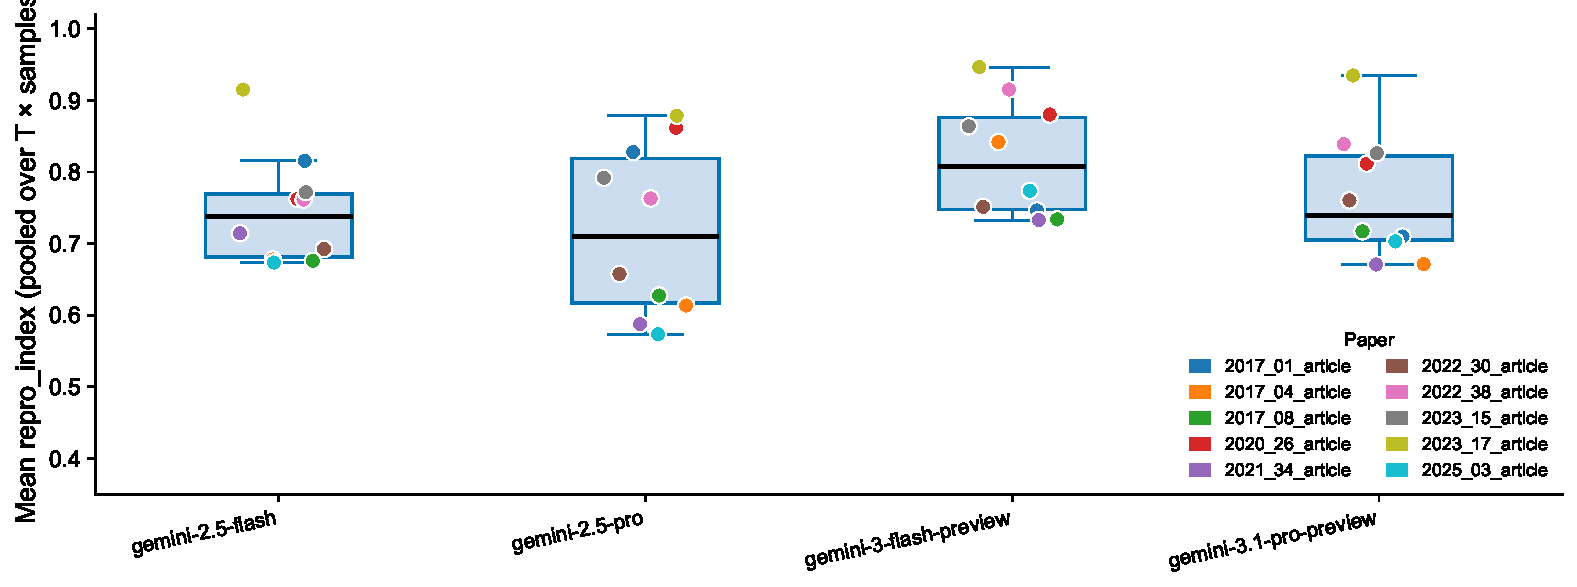
\includegraphics[width=\linewidth]{figures/fig1_model_comparison.pdf}
    \caption{Boxplot of mean repro\_index by model, pooled over temperatures and repeated runs for all evaluated papers.}
    \label{fig:fig1_model_comparison}
\end{figure}

Model performance is consistent across papers, with gemini-3-flash-preview achieving the highest repro\_index values (0.73--0.95), followed by gemini-3.1-pro-preview and gemini-2.5-flash, while gemini-2.5-pro and gpt-4.1 perform worse overall. Rankings remain stable regardless of paper length. Paper identity is the main source of variability: 2023\_17\_article is consistently the most reproducible (0.88--0.95), whereas 2025\_03\_article and 2017\_04\_article are the least reproducible (0.57--0.77), with within-model variation across papers exceeding differences between models.

To further examine the sources of variability, the effect of temperature on reproducibility was analysed for each model. Figure~\ref{fig:fig2_temperature_sensitivity} shows the standard deviation of the repro\_index across temperature settings, providing a measure of stability under different sampling conditions.

\begin{figure}[h]
    \centering
    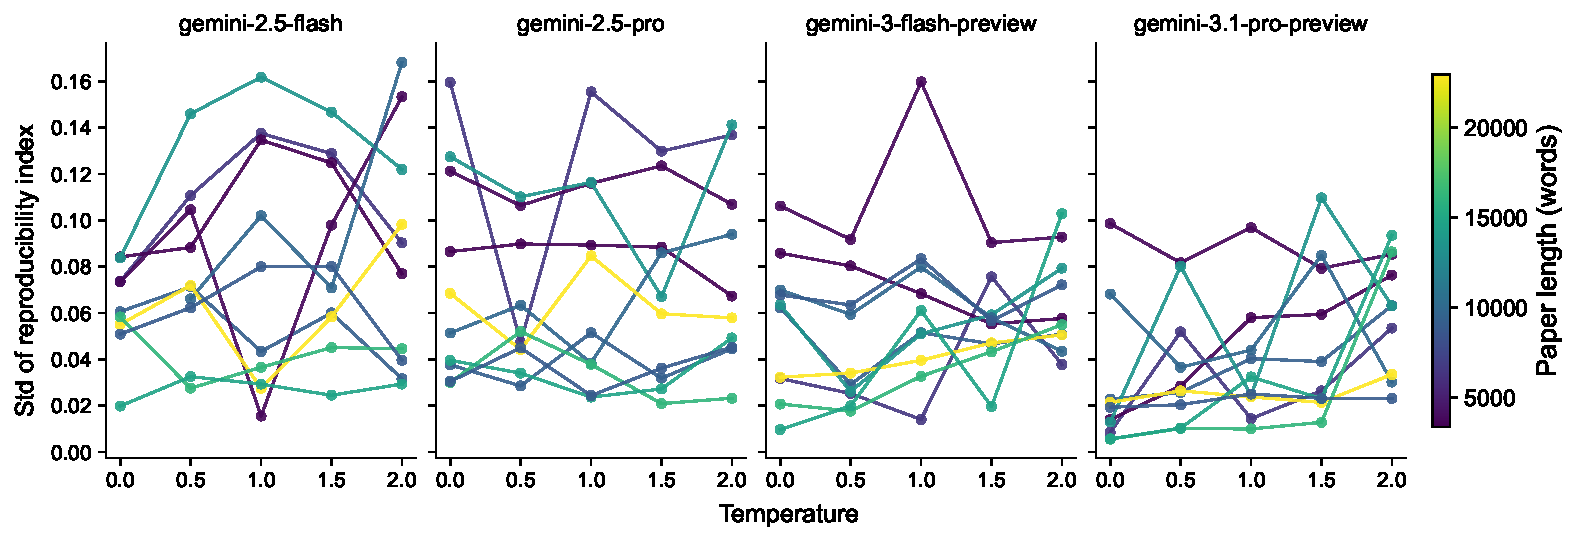
\includegraphics[width=\linewidth]{figures/fig2_temperature_sensitivity.pdf}
    \caption{Standard deviation of the repro\_index by temperature and model, indicating the sensitivity of each model to sampling variability.}
    \label{fig:fig2_temperature_sensitivity}
\end{figure}

The results indicate that temperature has a limited impact on the mean repro\_index but increases variability across runs. While the average score changes by less than 0.05 between $T=0$ and $T=2$ for most cases, the standard deviation rises from approximately 0.02--0.06 to 0.05--0.14. This suggests that the underlying scoring signal is robust to sampling noise at moderate temperatures, whereas higher temperatures introduce less reliable extractions.

No systematic relationship is observed between paper length and reproducibility. The repro\_index does not exhibit a monotonic trend with increasing document length, and variability is instead driven by paper-specific characteristics. For example, 2023\_17\_article (14\,733 words) yields the highest reproducibility, while longer papers such as 2022\_38\_article (22\,917 words) fall within a mid-range. One could argue that there is an optimum article length; Short papers need to be concise and therefore omitting some aspects, whereas longer ones could become too broad and dilute the key messages. Such an examination is out of the scope of the current work, but it could be the focus of future research.

Temperature effects on graph structure are model-dependent. For some models, particularly gemini-2.5-pro, higher temperatures lead to increased counts of sources, processes, and sinks, indicating over-decomposition of the workflow graph. In contrast, gemini-3.1-pro-preview remains comparatively stable across temperature settings. It should be noted that failure rates depend on both model and temperature. Failures cluster at higher temperatures, with gemini-2.5-pro exhibiting the highest failure frequency at $T=2$ indicating that that elevated stochasticity reduces robustness. Further analyses on the relationship between reproducibility, paper length, and graph structure are provided in Appendix~\ref{app:comparative-analyses}. These include results at $T=0$, where stochastic effects are minimised, as well as model-specific trends in node decomposition.

\subsection{Comparative Assessment} \label{comparative-assessment}

The current section focuses on a large-scale reproducibility evaluation using a single model, gemini-3.1-pro-preview, under deterministic conditions ($T=0$). The analysis covers all 213 ReScience-C articles published between 2015 and 2026, with one run per paper. This approach was selected to isolate variability due to document characteristics while removing stochastic effects from sampling. In order to characterise the relationship between structural extraction quality and semantic consistency under deterministic conditions, Figure~\ref{fig:structural_vs_content} presents a joint view of the structural score and content score for all 213 papers. The reproducibility index is encoded as a colour scale, allowing the interaction between both components to be assessed across the full corpus.

\begin{figure}
\centering
\includegraphics[width=0.75\linewidth]{figures/gemini3_1_pro_T0_structural_vs_content.pdf}
\caption{Relationship between structural score and content score for 213 ReScience-C articles at $T=0$ using gemini-3.1-pro-preview. Colour indicates the repro\_index.}
\label{fig:structural_vs_content}
\end{figure}

The corpus-level reproducibility shows a mean repro\_index of 0.762 ($\sigma = 0.093$), with values ranging from 0.361 to 0.979. The distribution is approximately bell-shaped with a slight left skew, indicating a minority of poorly reproducible cases but no strong bimodality.

The structural score is consistently high (mean 0.864), suggesting that the model reliably reconstructs plausible workflow graphs across papers. In contrast, the content score is lower (mean 0.685), indicating reduced consistency in the semantic reconstruction of individual nodes. As a result, content acts as the limiting factor in overall performance.

Taking into consideration that the repro\_index is defined as $\sqrt{\text{structural} \times \text{content}}$, the higher structural scores are not sufficient to offset the lower content scores, and the composite metric is therefore primarily constrained by semantic reproducibility rather than graph construction quality. Additional analyses are provided in Appendix~\ref{app:supp-analyses-structure-metadata} to further characterise structural and metadata-related factors affecting reproducibility.


% Comparative Assessment:
    % Run on ReScience C, discuss how and why it comes to similar conclusions like humans

% --> Outcome: ARA performs well across different scientific domains, meaning it comes to human-alike conclusions
% --> Outcome2: when ARA and humans disagree

\subsection{Model Benchmarking}

% Benchmarking: 
    % Run on existing benchmarks and compare with scoring of humans & agents
        % reproscreener - Machine Learning - Gunderson Metrics (selection), see Table 1 in 2024_Bhaskar.pdf, multiple criteria
        % reprobench - Empiric Social Science - SSRP reproducibility metric (one value at the end)
        
        % comparison score: either accuracy, or confusion matrix, or spearkman correlation rank
        % what could make sense is not to directly compare our assessment with theirs, but run a regression / ML classification model from our scores to theirs

% --> Outcome: Also on established benchmarks with different reproducibility scoring, ARA comes to similar conclusions like human assessments, and even better than the methods "reproscreener" and "reprobench"

\subsection{Agentic Resources Consumption}

%%%%%%%%%%%%%%%%%%%%%%%%%%%%%%%%%%%%%%%%%%%%%%%%%%%%
\section{Conclusion}
% Quick Summary of the work:
    %
    
% Discussion:
    % breaking down graph workflow of paper superior than just checklist-based document parsing
    % graph workflow enough to assess reproducibility, no need to actually reproduce in many cases
    % potential / vision: how ARA can help to support and scale review processes and impact peer-review and research in general
    
% Limitations:
    %
    
% Future Works:
    % Extend this to reproducing, not only reproducibility assessment    
    % Extend to citation grpahs, validity of citations, and referneces


\include{abbreviations}

%%%%%%%%%%%%%%%%%%%%%%%%%%%%%%%%%%%%%%%%%%%%%%%%%%%%
% \section*{References}


% References follow the acknowledgments in the camera-ready paper. Use unnumbered first-level heading for
% the references. Any choice of citation style is acceptable as long as you are
% consistent. It is permissible to reduce the font size to \verb+small+ (9 point)
% when listing the references.
% Note that the Reference section does not count towards the page limit.
% \medskip
\newpage
\bibliographystyle{IEEEtran}
% \bibliographystyle{plainnat}

\bibliography{references}


%%%%%%%%%%%%%%%%%%%%%%%%%%%%%%%%%%%%%%%%%%%%%%%%%%%%%%%%%%%%
\clearpage
\appendix

%\section{Technical appendices and supplementary material}
%Technical appendices with additional results, figures, graphs, and proofs may be submitted with the paper submission before the full submission deadline (see above). You can upload a ZIP file for videos or code, but do not upload a separate PDF file for the appendix. There is no page limit for the technical appendices. 

%Note: Think of the appendix as ``optional reading'' for reviewers. The paper must be able to stand alone without the appendix; for example, adding critical experiments that support the main claims to an appendix is inappropriate. 



%%%%%%%%%%%%%%%%%%%%%%%%%%%%%%%%%%%%%%%%%%%%%%%%%%%%%%%%%%%%%%%%%%%%%%%%%%%%%
\clearpage
\section{Appendix: Exemplary Scientific Workflow Graph} \label{appendix:ex_workflow}

Here, we provide an exemplary workflow generation for the work entitled \textit{"A Deep Reinforcement Learning Approach for Ramp Metering Based on Traffic Video Data"} from Bing et al. 2012 (doi: \href{https://doi.org/10.1155/2021/6669028}{10.1155/2021/6669028}) to illustrate the functioning of \texttt{ARA}.
This paper leverages real-world traffic data to generate a traffic simulation that is used to train a reinforcement-learning based controller, and its workflow graph is illustrated in the Figure~\ref{fig:example_workflow} below.

\texttt{ARA} distills source, method, experiment, and sink nodes, and their relationship (connection) from the document. 
Furthermore, the pipeline successfully identifies relevant sinks (actual results and outcomes of the research paper), while excluding irrelevant figures and tables (that rather serve for conceptual explanation or literature review purposes) from the analysis.

\begin{figure}[!h]
    \centering
    
\includegraphics[width=\linewidth]{figures/Example_Workflow.pdf}
    \caption{Workflow Graph Generated From A Scientific Paper.}
    \label{fig:example_workflow}
\end{figure}

The graph is stored in a Java-Script Notation Object (JSON) format as illustrated below. The general output structure comprises:
\begin{lstlisting}
{
  "metadata": { ... },
  "nodes_source": [ ... ],
  "nodes_process": [ ... ],
  "nodes_sink": [ ... ]
}
\end{lstlisting}

\newpage
The \textit{'metdata'} list comprises various general information about the publication, as well as a comprehensive list of \textit{'hyperparameters'}.
\begin{figure}[ht]
\noindent
\begin{minipage}[t]{0.6\textwidth}
\begin{lstlisting}[basicstyle=\ttfamily\small, frame=single]
"metadata": {
  "pdf_path": "...pdf",
  "extraction_model": "gemini-3.1-pro-preview",
  "title": "...",
  "authors": [ ... ],
  "repository_links": [ ... ],
  "supplementary_materials": [ ... ],
  "hyperparameters": [ ... ],
  "stated_software_versions": { ... },
  "hardware_requirements": null
},
\end{lstlisting}
\end{minipage}\hfill
\begin{minipage}[t]{0.39\textwidth}
\begin{lstlisting}[basicstyle=\ttfamily\small, frame=single]
"hyperparameters": [
  {
    "name": "...",
    "value": "...",
    "context": "...",
    "source_quote": "..."
  },
  ...
],
\end{lstlisting}
\end{minipage}
\end{figure}

\FloatBarrier

The \textit{'nodes\_process'} list comprises process nodes of type "method" and "experiment", while \textit{'nodes\_sink'} comprises nodes of type "figure" and "table".

\begin{figure}[!ht]
\noindent
\begin{minipage}[t]{0.49\textwidth}
\begin{lstlisting}[basicstyle=\ttfamily\small, frame=single]
"nodes_process": [
  {
    "node_id": "...",
    "node_name": "...",
    "source_quote": "...",
    "description": "...",
    "process_type": "method",
    "input_ids": [ ... ],
    "outcomes": [ ... ],
    "algorithm_clarity": 3,
    "tools_required": [ ... ],
    "tools_mentioned": [ ... ],
    "parameters_required": [ ... ],
    "parameters_mentioned": [ ... ],
    "reproducibility_score": 80,
    "reproducibility_rationale": "..."
  },
  ...
  {
    "node_id": "...",
    "node_name": "...",
    "source_quote": "...",
    "description": "...",
    "process_type": "experiment",
    "input_ids": [ ... ],
    "outcomes": [ ... ],
    "algorithm_clarity": 4,
    "tools_required": [ ... ],
    "tools_mentioned": [ .. ],
    "parameters_required": [ ... ],
    "parameters_mentioned": [ ... ],
    "reproducibility_score": 90,
    "reproducibility_rationale": "..."
  },
  ...
],
\end{lstlisting}
\end{minipage}\hfill
\begin{minipage}[t]{0.49\textwidth}
\begin{lstlisting}[basicstyle=\ttfamily\small, frame=single]
"nodes_sink": [
  {
    "node_id": "...",
    "node_name": "...",
    "source_quote": "...",
    "description": "...",
    "input_ids": [ ... ],
    "size_estimate": "...",
    "type": "figure",
    "statement_clarity": 3,
    "statement_validity": "...",
    "reproducibility_score": 85,
    "reproducibility_rationale": "..."
  },
  ...
  {
    "node_id": "...",
    "node_name": "...",
    "source_quote": "...",
    "description": "...",
    "input_ids": [ ... ],
    "size_estimate": "...",
    "type": "table",
    "statement_clarity": 4,
    "statement_validity": "...",
    "reproducibility_score": 85,
    "reproducibility_rationale": "..."
  },
  ...
],
\end{lstlisting}
\end{minipage}
\end{figure}




%%%%%%%%%%%%%%%%%%%%%%%%%%%%%%%%%%%%%%%%%%%%%%%%%%%%%%%%%%%%%%%%%%%%%%%%%%%%%
\clearpage
\section{Appendix: Prompt Templates} \label{appendix:prompts}

This appendix lists, verbatim, the prompts driving the structured extraction pipeline implemented in \texttt{src/ara\_pipeline/gemini\_rag.py}. The pipeline issues six queries per paper, all sharing one system instruction
(\ref{app:prompts:system}). Two of the six prompts are built at call time
(\ref{app:prompts:sink-nodes}, \ref{app:prompts:process-nodes}): the
canonical \texttt{src\_*} and \texttt{sink\_*} identifiers extracted by earlier queries are pasted into the prompt text so cross-layer wiring is resolved by exact string match. Execution order is: \texttt{header}
$\rightarrow$ \texttt{nodes\_source} $\rightarrow$ \texttt{nodes\_sink}
$\rightarrow$ \texttt{nodes\_process} $\rightarrow$ \texttt{artefacts}
$\rightarrow$ \texttt{parameters}.

\subsection{System instruction (shared by every query)}
\label{app:prompts:system}

\begin{lstlisting}
You are analysing a research paper for reproducibility. Answer using ONLY information explicitly stated in the attached PDF. If a fact is not stated, use null / omit it -- do NOT infer, guess, or draw on outside knowledge. Every item you extract must include a short literal quote from the paper that grounds it. Respond with valid JSON conforming to the provided schema; return nothing else.

BE TERSE. Avoid verbosity at all costs: do not restate the schema, do not add commentary, do not pad strings. Every string field is plain ASCII -- no combining diacritics, no non-BMP symbols, no long runs of repeated characters or tokens. Quotes are <=200 characters, descriptions <=400 characters, list items <=60 characters, lists <=8 items. If a field would exceed these limits, trim it; never produce filler to reach a limit. Close the JSON as soon as the required fields are populated -- truncation is a parse error.
\end{lstlisting}

\subsection{Header prompt (metadata)}
\label{app:prompts:header}

\begin{lstlisting}
Extract the paper's title and author list. If either is not clearly printed on the first page, use an empty string or empty list.
\end{lstlisting}

\subsection{Source nodes prompt (datasets)}
\label{app:prompts:source-nodes}

\begin{lstlisting}
List every dataset referenced in this paper. For each dataset, emit an object with these fields (in this order):
  * node_id                    -- canonical 'src_<slug>' id (rules below)
  * node_name                  -- human-readable dataset name as printed in the paper
  * source_quote               -- short literal quote (<=200 chars) anchoring the dataset
  * description                -- description of contents (<=400 chars)
  * size_estimate              -- approximate size (string) if stated, else null
  * license                    -- licence string if stated, else null
  * availability               -- 'open', 'upon_request', or 'not_mentioned'
  * url                        -- URL or DOI if provided, else null
  * reproducibility_score      -- INTEGER percentage in [0, 100] (rubric below)
  * reproducibility_rationale  -- short justification (<=200 chars) for that score

REPRODUCIBILITY SCORE RUBRIC (critical):
- 0   -- the dataset is referenced but is NOT available: no URL, no DOI, no repository, no acquisition path stated; or the paper marks it as 'not_mentioned'.
- 100 -- the dataset is openly mentioned with a concrete, working source (URL / DOI / public repository) that a third party can follow to obtain the exact dataset.
- Intermediate values reflect partial information, e.g.:
    * ~25  -- only a citation to a prior paper, no URL or repository;
    * ~50  -- access 'upon request' from authors, no public link;
    * ~75  -- public repository named (e.g. 'available on Zenodo') but no direct URL / DOI given.
Always set 'reproducibility_rationale' to a short string citing the specific facts that drove the score (e.g. 'open URL provided', 'citation-only, no DOI', 'upon-request, no link'). Anchor the score in what is actually stated in the paper -- do not infer availability from outside knowledge.

NODE ID RULES (critical):
- 'node_id' is used verbatim by nodes_process[*].input_ids to wire sources into the workflow graph, so format and stability matter.
- Format: 'src_<slug>' where <slug> is lowercase ASCII, digits and underscores only, max 40 chars, derived from the most specific noun phrase naming this dataset in the paper (NOT from description or license). Examples: 'src_adni_t1', 'src_synthetic_reward_traces', 'src_mnist'. Do not include the year, version, or author name unless the paper uses it as part of the dataset's primary name.
- node_id MUST be unique across the returned list.
- Keep node_id stable: for the same dataset in the same paper, the same slug should be emitted every run.
\end{lstlisting}

\subsection{Sink nodes prompt (results-bearing figures and tables)}
\label{app:prompts:sink-nodes}

This prompt is built at call time by \texttt{build\_sink\_nodes\_prompt(source\_ids)};
the \texttt{SOURCE IDS} block is filled with the \texttt{src\_*} identifiers
returned by the source-nodes query.

\begin{lstlisting}
List ONLY the figures and tables that REPORT RESULTS of the study. Emit a sink_node ONLY for an artefact that presents an outcome, measurement, evaluation, comparison, or finding produced BY the paper's methodology -- the kind of artefact a replication would have to recompute to claim the result was reproduced.

EXCLUDE (do NOT emit a sink_node for these):
  * methodology / architecture diagrams, schematics, flowcharts, pipelines, conceptual figures, illustrative cartoons;
  * tables that list hyperparameters, configuration values, network architecture, dataset statistics, parameter ranges, software versions, hardware specifications, symbol/notation glossaries, or experimental setup;
  * tables of related work, summaries of prior literature, or comparisons of methods that predate the paper's contribution;
  * sample / qualitative example figures that show inputs rather than outcomes; legend or colour-key panels.
If unsure whether an artefact is a result, ask: 'Does this report a MEASURED OUTCOME of the study?' If no, EXCLUDE it. Information from excluded tables/figures (parameter values, methodology details) is captured downstream by the nodes_process extraction; do NOT duplicate it here.

For each remaining results-bearing figure or table, emit a single sink_node object with these fields:
  * node_id            -- canonical 'sink_fig<N>' or 'sink_tab<N>' (rules below)
  * node_name          -- the paper's printed label, e.g. 'Figure 3', 'Table 1'
  * source_quote       -- short literal quote (<=200 chars) from the caption or prose
  * description        -- what the figure/table shows or presents (<=400 chars)
  * input_ids          -- predecessor labels (rules below)
  * size_estimate      -- approximate size if stated (e.g. 'N=120 cells x 6 columns', '8 panels'), else null
  * type               -- 'figure' or 'table'
  * statement_clarity  -- ordinal reconstructability score r(.) on a 4-level scale (BARE INTEGER in {1, 2, 3, 4}):
      1 -- MISSING information: only the artefact is shown; no procedure or inputs are described.
      2 -- PARTIAL: the procedure is named with some detail, but at least one required input or step is absent or only loosely described.
      3 -- MOSTLY SPECIFIED: most steps and inputs are stated; minor gaps remain (e.g. an unstated default, an ambiguous parameter).
      4 -- SUFFICIENT detail for independent reconstruction: every step FROM 'input_ids' TO this artefact is stated precisely enough to reimplement without guessing.
  * statement_validity -- one of:
      'supported'            -- claims directly justified by the listed inputs;
      'partially_supported'  -- some claims justified, others not;
      'unsupported'          -- conclusions exceed what the inputs can support;
      'not_assessed'         -- insufficient information to judge.
  * reproducibility_score      -- INTEGER percentage in [0, 100] (rubric below)
  * reproducibility_rationale  -- short justification (<=200 chars) for that score

REPRODUCIBILITY SCORE RUBRIC (critical):
The score combines TWO factors:
  (a) UPSTREAM REPRODUCIBILITY -- how openly stated, traceable, and parameterised the sources and method steps feeding 'input_ids' are (raw datasets cited with URL/DOI? methods specified clearly? parameter values stated? tools named?). Treat this as the SUM / AGGREGATE of the upstream nodes that produce the inputs to this artefact: weak inputs cap the achievable score.
  (b) DESCRIPTION COHERENCE -- how well the figure/table's stated result follows from those inputs. A well-described result that cleanly aggregates / visualises its inputs scores high; a result that introduces unexplained data, missing intermediate steps, or claims beyond what the inputs can yield scores low.
Anchors:
  * 0   -- inputs are unavailable / unspecified, OR the artefact's claim does not follow from them.
  * 100 -- every input is fully reproducible (open data, fully specified methods) AND the claim follows directly and coherently from those inputs.
  * Intermediate values reflect partial information, e.g.:
      ~25 -- some inputs cited but not retrievable; coherence weak;
      ~50 -- about half of the upstream chain is reproducible and the result is plausibly derivable;
      ~75 -- inputs mostly reproducible and the result follows clearly, with only minor unstated steps.
Treat the score as a GEOMETRIC integration of (a) and (b) -- if either is near zero (unavailable inputs OR incoherent claim) the score should be near zero. Always set 'reproducibility_rationale' to a short string citing the specific upstream gaps and any input-vs-claim coherence issues that drove the value (e.g. 'inputs cited only, coherent claim', 'inputs open + URL, claim aggregates them directly', 'one input missing, claim partially supported').

NODE ID RULES (critical):
- Each figure: 'sink_fig<N>' (e.g. 'sink_fig3', 'sink_fig3a' for sub-panels).
- Each table:  'sink_tab<N>' (e.g. 'sink_tab1').
- node_id MUST be unique across the returned list.

INPUT ID RULES (critical):
- 'input_ids' lists the immediate predecessor artefacts the figure or table is built from (lists <=8 items, each <=60 characters).
- Use the source ids below VERBATIM whenever the artefact draws directly on a raw dataset.
- Otherwise use a short lowercase snake_case label that a method step would naturally emit (e.g. 'metrics_<dataset>', 'predictions_<dataset>', 'features_<dataset>'). Downstream method extraction will reuse these labels.

SOURCE IDS -- use these verbatim in 'input_ids' whenever the figure/table consumes a raw dataset:
  - <src_id_1>
  - <src_id_2>
  - ...

OUTPUT-SIZE LIMITS (hard):
- All strings plain ASCII; no combining diacritics or non-BMP symbols.
- 'source_quote' <=200 chars; 'description' <=400 chars; 'node_name' <=8 words.
\end{lstlisting}


\subsection{Process nodes prompt (workflow steps)}
\label{app:prompts:process-nodes}

This prompt is built at call time by
\texttt{build\_process\_nodes\_prompt(source\_ids, sink\_ids)}; the
\texttt{SOURCE IDS} and \texttt{SINK IDS} blocks are filled with the
identifiers returned by the source- and sink-nodes queries.

\begin{lstlisting}
List every step of the research workflow in sequential execution order. Each step is a 'process node'; classify it as either a method (algorithmic / computational procedure) or an experiment (controlled trial, evaluation, ablation, comparison, sweep). Assign each step a canonical 'node_id' of the form 'meth_<NN>' with a zero-padded two-digit ordinal, starting at 'meth_01' and incrementing by 1 for each subsequent step. Also provide a short 'node_name' (<=8 words) and a 'description' of what the step does. Include a short literal quote (source_quote) anchoring each step.

OUTPUT-SIZE LIMITS (hard):
- Every field is plain ASCII. Do NOT emit combining diacritics, non-BMP symbols, or long runs of repeated characters.
- 'source_quote': <=200 characters, a single literal sentence fragment copied verbatim from the PDF.
- 'description': <=400 characters.
- 'node_name': <=8 words.
- Each list ('input_ids', 'outcomes', 'tools_required', 'tools_mentioned', 'parameters_required', 'parameters_mentioned') has at most 8 items; each item is <=60 characters.
- Never repeat the same token more than twice in a row. If you are near a field limit, stop and close the JSON -- truncation is a parse error.

FIELD SEMANTICS:
- 'process_type': one of
    * 'method'     -- an algorithmic or computational procedure (e.g. preprocessing, feature extraction, model training, inference, optimisation, simulation step);
    * 'experiment' -- a controlled trial that produces measured outcomes (e.g. evaluation on a held-out set, ablation study, hyperparameter sweep, baseline comparison, statistical test).
- 'input_ids': labels consumed by this step (source ids, sink ids, or verbatim labels emitted by earlier steps' 'outcomes').
- 'outcomes': labels produced by this step. Most are INTERMEDIATE artefacts consumed by a later step (partitions, preprocessed data, features, trained models, prediction tensors, metrics, etc.). Only the FINAL step(s) in a chain emit a sink id. A step may emit multiple outcomes: any number of intermediates plus at most one sink id.
- 'tools_required': the GENERIC technique / capability needed to execute the step (e.g. 'gradient-boosted classifier', 'stratified k-fold cross-validation', '2-D convolutional encoder'). State these even if the paper does not name a concrete library.
- 'tools_mentioned': CONCRETE tools / libraries / frameworks the paper explicitly names for this step, with version numbers when stated (append 'version not stated' otherwise). Leave empty if the paper does not name a tool for this step.
- 'parameters_required': names of parameters the technique NEEDS to be reproducible (e.g. 'learning_rate', 'batch_size', 'random_seed', 'n_estimators'), regardless of whether the paper provides a value. Use lowercase snake_case parameter names.
- 'parameters_mentioned': parameters the paper actually states for this step, as 'name=value' strings (e.g. 'learning_rate=1e-3', 'n_folds=5'). Only include parameters whose value is explicitly stated in the paper.
  IMPORTANT: tables and figures that are NOT results (e.g. tables of hyperparameters, configuration tables, architecture diagrams, notation glossaries, dataset-statistics tables, methodology flowcharts) are NOT nodes_sink -- they are part of the methodology specification. MINE them: extract every parameter value listed in such tables into 'parameters_mentioned' of the step that uses the parameter, fold any algorithmic detail shown in such figures into the step's 'description', and add any tool / library named there to 'tools_mentioned'. Anchor each extracted fact with a 'source_quote' from the table caption, table cell, or figure caption.
- 'algorithm_clarity': ordinal reconstructability score r(.) on a 4-level scale (integer in {1, 2, 3, 4}):
    * 1 -- MISSING information: the paper names the step but provides no algorithmic detail, no inputs, and no parameter values.
    * 2 -- PARTIAL specification: the algorithm is named with some detail, but at least one required input or parameter is absent or only loosely described.
    * 3 -- MOSTLY SPECIFIED components: most algorithmic choices, inputs, and required parameters are stated; minor gaps remain (e.g. an unstated default, an ambiguous tie-break).
    * 4 -- SUFFICIENT detail for independent reconstruction: the step's algorithm, inputs, and all required parameters are stated precisely enough to reimplement without guessing.
  Emit the BARE INTEGER (1, 2, 3, or 4) -- not a string.
- 'reproducibility_score': INTEGER percentage in [0, 100] derived from the four fields above, per this rubric:
    * 0   -- 'algorithm_clarity'=1 AND no tools / parameters listed.
    * 100 -- 'algorithm_clarity'=4 AND every item in 'tools_required' also appears in 'tools_mentioned' AND every item in 'parameters_required' has a value in 'parameters_mentioned'.
    * Intermediate values reflect partial specification. Suggested anchors:
        ~25 -- 'algorithm_clarity'=2 with most tools / parameters missing;
        ~50 -- 'algorithm_clarity'=3 with about half the tools / parameters named;
        ~75 -- 'algorithm_clarity'=3-4 with most tools named and most parameter values stated, only minor gaps remain.
  Treat the score as the GEOMETRIC integration of (clarity / 4), (tools_named_ratio), and (params_valued_ratio) -- if any of the three is zero, the score should be near zero. Do not round to a flat 50 when the inputs disagree.
- 'reproducibility_rationale': short string (<=200 chars) citing the concrete gaps that drove the score, e.g. 'clarity=3, 1/2 tools named, 4/5 params stated' or 'clarity=4, all tools+params stated'.

SOURCE IDS -- use these verbatim in 'input_ids' whenever a step consumes a raw dataset. Do NOT use human-readable dataset names, and do NOT invent new 'src_*' ids:
  - <src_id_1>
  - <src_id_2>
  - ...

SINK IDS -- use these verbatim in 'outcomes' ONLY when the step's direct output IS one of the figures/tables reported in the paper (typically the last step in a chain). If the step produces an intermediate artefact that a later step will turn into a figure or table, DO NOT put a sink id on this step. Do NOT invent new 'sink_*' ids:
  - <sink_id_1>
  - <sink_id_2>
  - ...

OUTCOME NAMING TEMPLATES (critical):
When a step derives an artefact from a source dataset, name the outcome using these templates, where <slug> is the source node_id WITH THE 'src_' PREFIX REMOVED (e.g. for source 'src_adni_t1' use slug 'adni_t1'):
  * 'train_<slug>', 'val_<slug>', 'test_<slug>' for splits
  * 'preprocessed_<slug>' for cleaned / normalised data
  * 'features_<slug>' for extracted features
  * 'predictions_<slug>' for model outputs evaluated on that dataset
  * 'metrics_<slug>' for evaluation metrics computed over that dataset
If the paper uses a different but specific name for the artefact, you MAY use it; otherwise apply these templates so downstream steps can reference the artefact by a predictable name. Purely internal intermediates (not tied to any one source dataset) may use free-form lowercase snake_case names.

LABEL CONSISTENCY RULES (critical):
- Use the SAME label for the same artefact across steps. If step N produces an outcome that feeds step N+1, the string in step N's 'outcomes' MUST appear verbatim in step N+1's 'input_ids'. Do not paraphrase, pluralise, or reorder words between steps; pick one canonical name per artefact and reuse it.
- When a step splits, partitions, or divides a dataset (e.g. train/test split, k-fold, train/val/test, stratified sampling), 'outcomes' MUST list each resulting partition as a separate named item using the 'train_<slug>' / 'val_<slug>' / 'test_<slug>' templates above (use whatever names the paper uses if stated). The 'description' MUST state the split percentages / proportions / fold count exactly as reported in the paper (e.g. '80/20 split', '70/15/15', '5-fold cross-validation'). Downstream steps that consume a partition MUST reference it by the same name in 'input_ids'.
\end{lstlisting}

\subsection{Artefacts prompt (code, supplements, hardware) (metadata)}
\label{app:prompts:artefacts}

\begin{lstlisting}
List all code repositories, supplementary materials, and external resources mentioned anywhere in this paper -- references, footnotes, acknowledgements, data availability statement. Include URLs, GitHub links, Zenodo DOIs, and institutional repository references. Also state any stated hardware requirements.
\end{lstlisting}

\subsection{Parameters prompt (hyperparameters, software, hardware) (metadata)}
\label{app:prompts:parameters}

\begin{lstlisting}
List all parameters, hyperparameters, configuration values, and hardware requirements mentioned in this paper. Include numerical values, ranges, and any stated defaults. Return software versions as a list of objects, each with 'name' and 'version' fields.
\end{lstlisting}




%%%%%%%%%%%%%%%%%%%%%%%%%%%%%%%%%%%%%%%%%%%%%%%%%%%%%%%%%%%%%%%%%%%%%%%%%%%%%
\clearpage
\section{Appendix: Benchmarks \& Datasets} \label{appendix:benchmarks}

This subsection describes the benchmark datasets used to evaluate our reproducibility assessment framework. 
We rely on three complementary resources that span different scientific domains, annotation schemes, and levels of granularity: \textit{Reproscreener}~\citep{bhaskar2024reproscreener}, \textit{Repro-Bench}~\citep{hu2025repro}, and the \textit{ReScience~C} corpus~\citep{rougier2018rescience}. 
Together, these datasets provide manually curated ground-truth reproducibility annotations derived from expert assessments and reproduction reports, enabling evaluation across both binary and ordinal scoring settings. 
Table~\ref{tab:dataset_comparison} summarizes their key characteristics, and the following subsections describe each dataset in more detail.

\begin{table}[!h]
\renewcommand{\tabularxcolumn}[1]{>{\raggedright\arraybackslash}p{#1}}
\centering
\caption{\textbf{Reproducibility Assessment Benchmark Datasets.} This table summarizes and contrasts three major reproducibility assessment benchmark datasets used in this study.}
\label{tab:dataset_comparison}
\small
\begin{tabularx}{\linewidth}{lXXX}
\toprule
    \textbf{Criterion} & \textbf{Reproscreener}~\citep{bhaskar2024reproscreener} & \textbf{Repro-Bench}~\citep{hu2025repro} & \mbox{\textbf{ReScience C}~\citep{rougier2018rescience} (this work)} \\
    \midrule
    
    Size (\# papers)
    & 50
    & 112
    & 215
    \\
    
    Time-span
    & 2021--2022
    & 2019--2024
    & 2015--2026
    \\
    
    Domain
    & Machine Learning
    & Social Sciences
    & Multi-Domain
    \\
    
    Reproducibility
    \\
    
    \makecell[tl]{\;\;\;\; Scale}
    & Binary (0 / 1)
    & Ordinal (1--4)
    & Ordinal (1--4)
    \\
    
    \makecell[t]{\;\;\;\; Dimensions}
    & \makecell[tl]{Gunderson metrics~\citep{gundersen2018state}\\ objective, method,\\dataset, hypothesis, \\prediction, code, setup)}
    & \makecell[tl]{Total Score}
    & \makecell[tl]{Sources, Methods,\\Experiments, Sinks}
    \\
    
    Source
    & \makecell[tl]{arXiv preprints\\ (\texttt{cs.LG}, \texttt{stat.ML})}
    & \makecell[tl]{Mass reproduction study\\I4R discussion papers\\Retraction Watch database\\X (Twitter)}
    & \makecell[tl]{ReScience C open-\\ access replication journal}
    \\
\bottomrule
\end{tabularx}
\end{table}

\subsection{Reproscreener}

The \textit{Reproscreener} dataset~\citep{bhaskar2024reproscreener} consists of 50 machine learning preprints sampled from arXiv, specifically drawn from the \texttt{cs.LG} and \texttt{stat.ML} categories, which represent the principal domains for machine learning research submissions on the platform. 
The preprints were selected using a controlled query restricted to manuscripts last updated between October 24 and October 25, 2022, comprising 50 manuscripts. 
Each paper was manually labeled by the authors with respect to a predefined set of binary reproducibility indicators derived from the Gunderson metrics~\citep{gundersen2018state}, including statements of (i) research problem, (ii) research objective, (iii) research method, (iv) dataset, (v) hypothesis, (vi) predictions, (vii) code availability, and (viii) experiment setup.

\subsection{Repro-Bench}

The \textit{Repro-Bench} dataset~\citep{hu2025repro} a curated benchmark consisting of 112 scientific works, each corresponding to a published social science paper accompanied with its publicly available (human generated) reproduction package and reproduction report. 
The dataset spans multiple subdomains of social science research and was constructed from four complementary sources: a \textit{large-scale mass reproduction effort}~\citep{brodeur2024mass} covering economics and political science papers (92 instances), the \textit{Institute for Replication (I4R) discussion paper series}~\citep{i4r} (11 instances), the\textit{ Retraction Watch database}~\citep{retrdb} (7 instances), and publicly documented reproduction analyses shared on \textit{X} (formerly \textit{Twitter}) (2 instances). 
Each paper satisfies strict inclusion criteria, including the availability of a DOI, an executable reproduction package (data, code, and documentation), and a credible expert-written reproduction report verifying computational results. 
Ground-truth reproducibility labels are derived directly from these reproduction reports and assigned using a four-level scoring scheme that reflects the consistency between reported findings and reproduced outputs: score~1 indicates irreproducible major findings, score~2 indicates minor coding inconsistencies without affecting conclusions, score~3 indicates minor reporting discrepancies (e.g., rounding differences), and score~4 indicates fully reproducible results. 
The annotation process follows a structured consensus-based protocol in which the lead author first assigns labels based on reproduction reports and a five-member expert team subsequently cross-validates all scores to ensure consistency~\citep{hu2025repro}. 

\subsection{ReScience C}

We additionally leverage the \textit{ReScience~C} corpus, a platinum open-access, peer-reviewed journal dedicated to the publication of reproducible replications of computational research \citep{rougier2018rescience}. 
ReScience~C specifically targets independent reimplementations of previously published studies and requires authors to provide complete open-source code, documentation, and replication reports verifying whether the original results can be reproduced. 
Unlike traditional journals, ReScience~C operates through an open and collaborative publishing workflow hosted on GitHub, where submissions, reviews, code execution checks, and revisions are conducted transparently and publicly. 
As of 2015–2026, the journal contains 215 published replication studies spanning multiple computational domains. 
Each article includes a human-generated reproduction report together with executable code and supporting materials, allowing direct verification of whether figures, tables, and claims from the target paper can be reproduced. 
These expert-written reproduction reports serve as ground-truth evidence for reproducibility assessments, making the corpus particularly suitable for benchmarking automated reproducibility evaluation methods.

Following \citep{hu2025repro} and \citep{brodeur2024mass}, we operationalize reproducibility as a structured, ordinal assessment reflecting the consistency between reported results and independently reproduced outputs. Specifically, we evaluate reproducibility on a four-level scale from 0 to 3 and measure reproducibility across four complementary dimensions that correspond to distinct stages of the evidence-generation pipeline (i) sources, (ii) methods, (iii) experiments, and (iv) sinks (results).
The labels are derived from the human generated reproducibility efforts, similar to~\citep{hu2025repro}.

\section{Appendix: Supplementary analyses on reproducibility and graph structure}
\label{app:repro_graph}

\subsection{Comparative analyses}
\label{app:comparative-analyses}

Thie current appendix provides additional analyses supporting the main results on reproducibility and model behaviour. Since temperature introduces stochastic variability in the generation process, all supplementary analyses are reported at $T=0$ unless otherwise stated, as this setting provides the most stable baseline for comparison.

Figure~\ref{fig:repro_vs_paper_length_T0} investigates the relationship between paper length and reproducibility at $T=0$ across models, allowing an assessment of whether document size systematically affects the repro\_index in the absence of sampling noise.

\begin{figure}[!h]
\centering
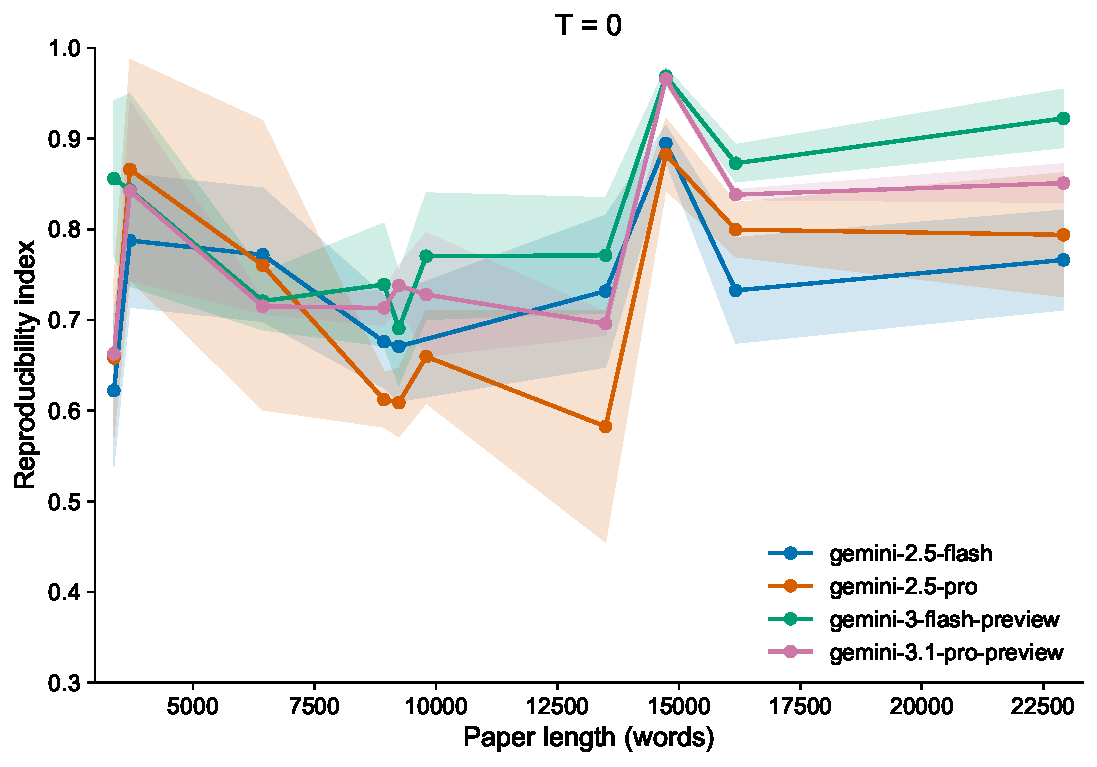
\includegraphics[width=\linewidth]{figures/repro_vs_paper_length_T0.pdf}
\caption{Repro\_index as a function of paper length at $T=0$, shown for each model.}
\label{fig:repro_vs_paper_length_T0}
\end{figure}

The dominant feature is a sharp peak at $\sim 14\,700$ words (2023\_17\_article), where all four models converge near 0.96--0.97 -- the single most reproducible paper in the consistency sweep. Outside that peak, the lines are non-monotonic and model-specific. The \texttt{gemini-2.5-pro} (orange) shows the most volatile trajectory, dropping to $\sim 0.58$--$0.61$ in the 9\,000--13\,000 word range before recovering, and its shaded std band is by far the widest, particularly in the mid-length region. The most stable model across all lengths is\texttt{gemini-3-flash-preview} (green) with a consistently high line and narrow band. In the mid-range, \texttt{gemini-2.5-flash} (blue) and \texttt{gemini-3.1-pro-preview} (pink) track each other closely. The right portion of the plot ($> 16\,000$ words) shows a gradual convergence of all models around 0.77--0.93, with \texttt{gemini-3-flash-preview} remaining highest. The key takeaway is that paper length alone is not a reliable predictor of reproducibility: the best and worst papers are both in the mid-length range, and the pattern is driven by individual paper characteristics rather than any length effect.

 Figure~\ref{fig:nodes_by_model_paper_length} further analyses how graph complexity evolves with paper length by decomposing the number of generated nodes into sources, processes, and sinks for each model. Together, these figures provide insight into whether observed differences in reproducibility and structure are driven by input size or model-specific behaviour.

\begin{figure}[!h]
\centering
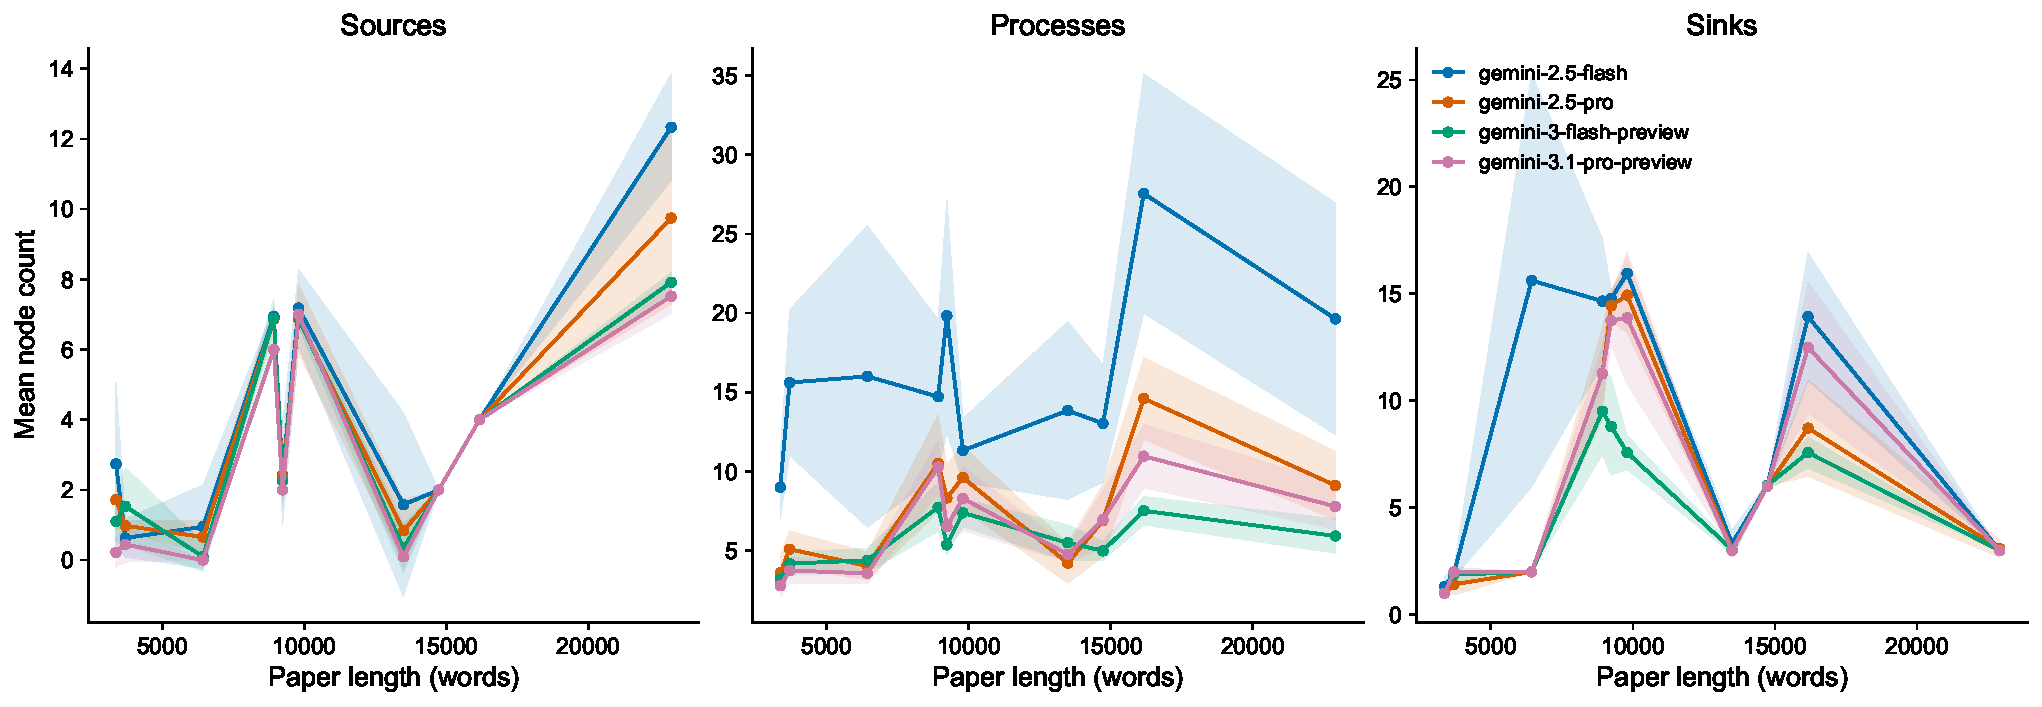
\includegraphics[width=\linewidth]{figures/nodes_by_model_paper_length.pdf}
\caption{Number of nodes (sources, processes, sinks) by paper length and model at $T=0$.}
\label{fig:nodes_by_model_paper_length}
\end{figure}

All three panels show a broadly increasing trend in node counts with paper length with a drop in the mid range. The \texttt{gemini-2.5-flash} (blue) is a consistent outlier across all three layers -- it extracts far more nodes than the other three models, especially for process nodes (reaching $\sim 27$ at 15\,700 words vs. $\sim 10$--$15$ for others) and sink nodes ($\sim 15$--$16$ in the 9\,000--10\,000 word range). This inflation likely reflects over-decomposition: the flash model splits workflow steps more finely. The three remaining models (gemini-2.5-pro, gemini-3-flash-preview, gemini-3.1-pro-preview) cluster tightly together with very similar node counts across all lengths, suggesting a shared decomposition style. Source nodes show a characteristic dip at $\sim 13\,000$ words before rising steeply at 22\,000+ words, consistent across all models. The wide shaded bands for \texttt{gemini-2.5-flash} in the process panel confirm high run-to-run variance for that model, particularly for longer papers.

\subsection{Supplementary analyses of structural, metadata, and temporal effects}
\label{app:supp-analyses-structure-metadata}

Most local connectivity properties are near-complete, with resolved inputs (0.993) and sink production (0.983) approaching unity, and a high largest weakly connected component fraction (0.865). In contrast, source-to-sink reachability is substantially lower (0.572), identifying it as the limiting structural factor. This indicates that while individual workflow components are well connected, end-to-end data flow from inputs to outputs is frequently incomplete, with approximately 43\% of cases lacking full connectivity. Figure~\ref{fig:gemini3_1_pro_T0_wiring_metrics} summarises the structural wiring metrics across the full corpus. 

\begin{figure}[!h]
\centering
\includegraphics[width=\linewidth]{figures/gemini3_1_pro_T0_wiring_metrics.pdf}
\caption{Structural wiring metrics across 213 ReScience-C papers. Mean ±std of the five wiring metrics used to compute the structural reproducibility score (gemini-3.1-pro-preview, $T =0$). Four of the five metrics exceed 0.81, reflecting that the LLM reliably connects process nodes to both data sources and result sinks. The exception is source-to-sink reachability (mean = 0.57, orange), which measures whether a directed path exists from every source node to at least one sink node. The gap indicates that workflow graphs frequently lack end-to-end connectivity — methods sections describe individual steps but do not trace a continuous data flow from raw inputs to published outputs.}
\label{fig:gemini3_1_pro_T0_wiring_metrics}
\end{figure}


Four bars cluster near 0.81--0.99: sinks produced (0.98) and resolved inputs (0.99) are near-perfect with very small error bars, while LWCC fraction (0.87) and sources consumed (0.81) are slightly lower but still strong. The orange source-to-sink reachability bar (0.57) stands in stark contrast, with an error bar spanning roughly 0.22--0.92 -- the highest variance of any metric. This wide spread indicates that end-to-end traceability is highly paper-specific: some papers provide complete source$\rightarrow$sink paths while others have none. The gap between 0.99 resolved inputs and 0.57 source-to-sink reachability is particularly telling: process steps cite their inputs correctly, but the overall data flow is not traced end-to-end.

 Papers providing a repository link ($n=152$) achieve a higher mean repro\_index (0.781) compared to those without ($n=61$, 0.714), corresponding to a +6.7 percentage point increase. While statistically significant (Mann--Whitney $p < 0.001$), this result indicates that code availability improves reproducibility but is not sufficient on its own. Figure~\ref{fig:code_availability} presents the effect of repository availability on reproducibility.

\begin{figure}[!h]
\centering
\includegraphics[width=\linewidth]{figures/gemini3_1_pro_T0_metadata_richness.pdf}
\caption{Effect of repository availability on repro\_index at $T=0$. Papers with code repositories show higher reproducibility (+6.7 pp; Mann--Whitney $p < 0.001$).}
\label{fig:code_availability}
\end{figure}

Left panel: papers with a repository link ($n = 152$, blue) have a visibly higher box than those without ($n = 61$, orange). The no-repo median is $\sim 0.72$ vs. $\sim 0.79$ for has-repo, and the no-repo distribution shows a longer lower tail with outliers reaching $\sim 0.36$. The *** significance annotation (Mann--Whitney $p < 0.001$) confirms that the difference is not due to sampling noise. Right panel: hyperparameter count shows $r = 0.018$, indicating a flat, circular cloud with no discernible trend. Most papers report 7--10 hyperparameters; higher counts do not correspond to higher reproducibility scores. This asymmetry between the two metadata predictors is noteworthy: repository presence is associated with higher reproducibility, while explicit parameter count is not informative.

Correlations between node counts and repro\_index are negligible across sources ($r=0.03$), processes ($r=0.13$), and sinks ($r=0.02$), indicating that larger graphs do not correspond to higher reproducibility. This suggests that descriptive quality and coherence, rather than graph size, determine reproducibility outcomes. Figure~\ref{fig:node_counts} examines the relationship between workflow graph size and reproducibility.

\begin{figure}[!h]
\centering
\includegraphics[width=\linewidth]{figures/gemini3_1_pro_T0_node_counts_vs_repro.pdf}
\caption{Relationship between node counts and repro\_index. No meaningful correlation is observed across sources, processes, or sinks ($r < 0.13$).}
\label{fig:node_counts}
\end{figure}

All three panels display circular, structureless clouds with source nodes ($r = 0.029$) and sink nodes ($r = 0.019$) being essentially uncorrelated with repro\_index. Process nodes ($r = 0.129$) show a marginally positive association -- the only panel with any visible trend -- but even this is negligible. Papers with only 1--2 source nodes span the full range from 0.36 to 0.98; the same is true for papers with 10+ nodes. The strong vertical clustering of source nodes at counts 1--5 reflects that most papers reference few datasets, while a long right tail of papers with 10--17 source nodes shows no corresponding gain in reproducibility. The conclusion is unambiguous: extracting more nodes does not produce a higher score and that reproducibility is determined by the quality of what is described, not the quantity.

The repro\_index remains broadly stable across publication years (2015--2023), with no clear monotonic trend. A local minimum is observed in 2017, likely reflecting potential early publication practices prior to the consolidation of editorial standards. Figure~\ref{fig:year_trend} presents reproducibility trends over time. 

\begin{figure}[!h]
\centering
\includegraphics[width=\linewidth]{figures/gemini3_1_pro_T0_repro_by_year.pdf}
\caption{Mean repro\_index by publication year (2015--2023). No clear temporal trend is observed; a dip occurs in 2017.}
\label{fig:year_trend}
\end{figure}

The mean line (orange) is broadly flat from 2016 to 2023 in the range 0.73--0.79, with two visible dips: 2017 (mean $\sim 0.65$, median $\sim 0.65$, and a low outlier near 0.36) and 2026 (mean $\sim 0.63$). The 2017 dip aligns with the early cohort of ReScience-C publications, while the 2026 dip likely reflects a small and potentially atypical sample. Box widths are similar across years from 2019 onward, indicating stable within-year variance. No upward trend is visible, which argues against a gradual improvement in reproducibility standards over time. The year 2024 is absent, as no papers are included for that period in the dataset.

The repro\_index spans a wide range from 0.361 to 0.979, indicating substantial heterogeneity. Top-ranked papers are consistently reproducible across analyses, with 2023\_17\_article appearing among the highest-scoring cases in both the consistency and full-corpus evaluations, supporting the robustness of the ranking. Figure~\ref{fig:paper_ranking} shows the distribution of reproducibility across individual papers.

\begin{figure}[!h]
\centering
\includegraphics[width=\linewidth]{figures/gemini3_1_pro_T0_paper_ranking.pdf}
\caption{Top and bottom 15 papers ranked by repro\_index. The range spans 0.361 to 0.979.}
\label{fig:paper_ranking}
\end{figure}

\subsection{Cross validation}
\label{app:cross-validation}

The top 15 papers (blue) form a tight cluster from $\sim 0.90$ to $0.98$, with \texttt{2020\_27\_article} at the top (0.979) and \texttt{2020\_36\_article} at the boundary ($\sim 0.90$). The bottom 15 (orange) are more dispersed, ranging from \texttt{2021\_26\_article} ($\sim 0.46$) and \texttt{2017\_09\_article} ($\sim 0.36$) at the extreme to \texttt{2020\_31\_article} ($\sim 0.65$) just below the median. The dashed median line (0.754) lies well above the bottom cluster, confirming that these papers are genuinely low in reproducibility rather than merely below average. A clear separation is visible between the top cluster ($\ge 0.90$) and the rest of the corpus, indicating that high-reproducibility papers form a distinct regime rather than a gradual extension of the distribution.

Figure~\ref{fig:cross_validation} compares multi-sample and single-run reproducibility estimates for the subset of papers shared between the consistency and full-corpus analyses. The results show strong agreement between both evaluation approaches.

\begin{figure}[!h]
\centering
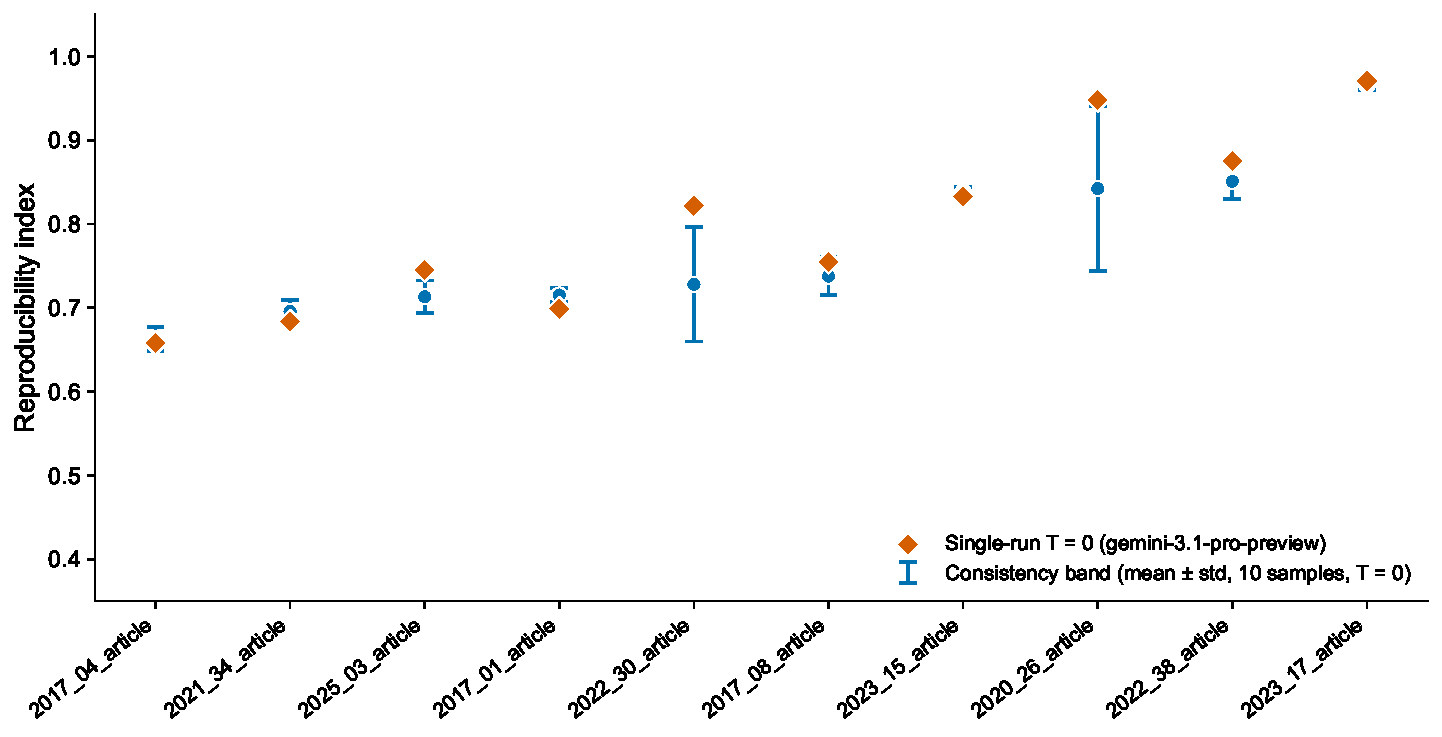
\includegraphics[width=\linewidth]{figures/fig8_cross_validation.pdf}
\caption{Cross-dataset validation of single-run $T=0$ scoring. Comparison of multi-sample ($n=10$, blue error bars) and single-run (orange diamonds) repro\_index for 10 shared papers. Papers are ordered by the multi-sample mean. Five of ten single-run values fall within $\pm 1$ standard deviation, and all fall within $\pm 2$ standard deviations, indicating strong agreement between both evaluation protocols.}
\label{fig:cross_validation}
\end{figure}


The orange diamonds (single-run $T=0$) closely follow the blue consistency bands (mean $\pm 1$ std, 10 samples) for the lower-scoring papers on the left (2017\_04, 2021\_34, 2025\_03), where both estimates agree in the range 0.66--0.75. As reproducibility increases, discrepancies become more pronounced. In particular, 2020\_26 shows the largest deviation, with the single-run estimate ($\sim 0.94$) clearly exceeding the consistency mean ($\sim 0.84$), indicating sensitivity of this paper to sampling variability. A similar upward deviation is observed for 2022\_38 and 2023\_17, where single-run values are again higher than the multi-sample means.

Overall, single-run $T=0$ estimates tend to be slightly optimistic relative to the multi-sample baseline, but remain consistently bounded within $\pm 2$ standard deviations across all cases. This confirms that deterministic single-run evaluation provides a reliable approximation of the expected reproducibility score while introducing a small positive bias.


%%%%%%%%%%%%%%%%%%%%%%%%%%%%%%%%%%%%%%%%%%%%%%%%%%%%%%%%%%%%%%%%%%%%%%%%%%%%%
\clearpage
\section{Appendix: Pipeline}

\subsection{Graph Construction}

\begin{figure}[!h]
    \centering
    \includegraphics[width=\linewidth]{figures/grafik.png}
    \caption{Enter Caption}
    \label{fig:placeholder}
\end{figure}

\subsection{Micro Level Scoring}




%%%%%%%%%%%%%%%%%%%%%%%%%%%%%%%%%%%%%%%%%%%%%%%%%%%%%%%%%%%%
\clearpage
\newpage
\input{checklist.tex}


%%%%%%%%%%%%%%%%%%%%%%%%%%%%%%%%%%%%%%%%%%%%%%%%%%%%

% \section{Submission of papers to NeurIPS 2026}


% Please read the instructions below carefully and follow them faithfully.


% \subsection{Style}


% Papers to be submitted to NeurIPS 2026 must be prepared according to the
% instructions presented here. Papers may only be up to {\bf nine} pages long, including figures. \textbf{Papers that exceed the page limit will not be reviewed (or in any other way considered) for presentation at the conference.}
% Additional pages \emph{containing acknowledgments, references, checklist, and optional technical appendices} do not count as content pages. 


% The margins in 2026 are the same as those in previous years.


% Authors are required to use the NeurIPS \LaTeX{} style files obtainable at the NeurIPS website as indicated below. Please make sure you use the current files and not previous versions. Tweaking the style files may be grounds for desk rejection.


% \subsection{Retrieval of style files}


% The style files for NeurIPS and other conference information are available on the website at
% \begin{center}
%   \url{https://neurips.cc}.
% \end{center}
% % The file \verb+neurips_2026.pdf+ contains these instructions and illustrates the various formatting requirements your NeurIPS paper must satisfy.


% The only supported style file for NeurIPS 2026 is \verb+neurips_2026.sty+, rewritten for \LaTeXe{}. \textbf{Previous style files for \LaTeX{} 2.09,  Microsoft Word, and RTF are no longer supported.}


% The \LaTeX{} style file contains three optional arguments: 
% \begin{itemize}
% \item \verb+final+, which creates a camera-ready copy, 
% \item \verb+preprint+, which creates a preprint for submission to, e.g., arXiv, \item \verb+nonatbib+, which will not load the \verb+natbib+ package for you in case of package clash.
% \end{itemize}


% \paragraph{Preprint option}
% If you wish to post a preprint of your work online, e.g., on arXiv, using the NeurIPS style, please use the \verb+preprint+ option. This will create a nonanonymized version of your work with the text ``Preprint. Work in progress.'' in the footer. This version may be distributed as you see fit, as long as you do not say which conference it was submitted to. Please \textbf{do not} use the \verb+final+ option, which should \textbf{only} be used for papers accepted to NeurIPS.


% At submission time, please omit the \verb+final+ and \verb+preprint+ options. This will anonymize your submission and add line numbers to aid review. Please do \emph{not} refer to these line numbers in your paper as they will be removed during generation of camera-ready copies.


% The file \verb+neurips_2026.tex+ may be used as a ``shell'' for writing your paper. All you have to do is replace the author, title, abstract, and text of the paper with your own.


% The formatting instructions contained in these style files are summarized in Sections \ref{gen_inst}, \ref{headings}, and \ref{others} below.


% \section{General formatting instructions}
% \label{gen_inst}


% The text must be confined within a rectangle 5.5~inches (33~picas) wide and
% 9~inches (54~picas) long. The left margin is 1.5~inch (9~picas).  Use 10~point
% type with a vertical spacing (leading) of 11~points.  Times New Roman is the
% preferred typeface throughout, and will be selected for you by default.
% Paragraphs are separated by \nicefrac{1}{2}~line space (5.5 points), with no
% indentation.


% The paper title should be 17~point, initial caps/lower case, bold, centered
% between two horizontal rules. The top rule should be 4~points thick and the
% bottom rule should be 1~point thick. Allow \nicefrac{1}{4}~inch space above and
% below the title to rules. All pages should start at 1~inch (6~picas) from the
% top of the page.


% For the final version, authors' names are set in boldface, and each name is
% centered above the corresponding address. The lead author's name is to be listed
% first (left-most), and the co-authors' names (if different address) are set to
% follow. If there is only one co-author, list both author and co-author side by
% side.


% Please pay special attention to the instructions in Section \ref{others}
% regarding figures, tables, acknowledgments, and references.

% \section{Headings: first level}
% \label{headings}


% All headings should be lower case (except for first word and proper nouns),
% flush left, and bold.


% First-level headings should be in 12-point type.


% \subsection{Headings: second level}


% Second-level headings should be in 10-point type.


% \subsubsection{Headings: third level}


% Third-level headings should be in 10-point type.


% \paragraph{Paragraphs}


% There is also a \verb+\paragraph+ command available, which sets the heading in
% bold, flush left, and inline with the text, with the heading followed by 1\,em
% of space.


% \section{Citations, figures, tables, references}
% \label{others}


% These instructions apply to everyone.


% \subsection{Citations within the text}


% The \verb+natbib+ package will be loaded for you by default.  Citations may be
% author/year or numeric, as long as you maintain internal consistency.  As to the
% format of the references themselves, any style is acceptable as long as it is
% used consistently.


% The documentation for \verb+natbib+ may be found at
% \begin{center}
%   \url{http://mirrors.ctan.org/macros/latex/contrib/natbib/natnotes.pdf}
% \end{center}
% Of note is the command \verb+\citet+, which produces citations appropriate for
% use in inline text.  For example,
% \begin{verbatim}
%    \citet{hasselmo} investigated\dots
% \end{verbatim}
% produces
% \begin{quote}
%   Hasselmo, et al.\ (1995) investigated\dots
% \end{quote}


% If you wish to load the \verb+natbib+ package with options, you may add the
% following before loading the \verb+neurips_2026+ package:
% \begin{verbatim}
%    \PassOptionsToPackage{options}{natbib}
% \end{verbatim}


% If \verb+natbib+ clashes with another package you load, you can add the optional
% argument \verb+nonatbib+ when loading the style file:
% \begin{verbatim}
%    \usepackage[nonatbib]{neurips_2026}
% \end{verbatim}


% As submission is double blind, refer to your own published work in the third
% person. That is, use ``In the previous work of Jones et al.\ [4],'' not ``In our
% previous work [4].'' If you cite your other papers that are not widely available
% (e.g., a journal paper under review), use anonymous author names in the
% citation, e.g., an author of the form ``A.\ Anonymous'' and include a copy of the anonymized paper in the supplementary material.


% \subsection{Footnotes}


% Footnotes should be used sparingly.  If you do require a footnote, indicate
% footnotes with a number\footnote{Sample of the first footnote.} in the
% text. Place the footnotes at the bottom of the page on which they appear.
% Precede the footnote with a horizontal rule of 2~inches (12~picas).


% Note that footnotes are properly typeset \emph{after} punctuation
% marks.\footnote{As in this example.}


% \subsection{Figures}


% \begin{figure}
%   \centering
%   \fbox{\rule[-.5cm]{0cm}{4cm} \rule[-.5cm]{4cm}{0cm}}
%   \caption{Sample figure caption. Explain what the figure shows and add a key take-away message to the caption.}
% \end{figure}


% All artwork must be neat, clean, and legible. Lines should be dark enough for
%  reproduction purposes. The figure number and caption always appear after the
% figure. Place one line space before the figure caption and one line space after
% the figure. The figure caption should be lower case (except for the first word and proper nouns); figures are numbered consecutively.


% You may use color figures.  However, it is best for the figure captions and the
% paper body to be legible if the paper is printed in either black/white or in
% color.


% \subsection{Tables}


% All tables must be centered, neat, clean, and legible.  The table number and
% title always appear before the table.  See Table~\ref{sample-table}.


% Place one line space before the table title, one line space after the
% table title, and one line space after the table. The table title must
% be lower case (except for the first word and proper nouns); tables are
% numbered consecutively.


% Note that publication-quality tables \emph{do not contain vertical rules}. We
% strongly suggest the use of the \verb+booktabs+ package, which allows for
% typesetting high-quality, professional tables:
% \begin{center}
%   \url{https://www.ctan.org/pkg/booktabs}
% \end{center}
% This package was used to typeset Table~\ref{sample-table}.


% \begin{table}
%   \caption{Sample table caption. Explain what the table shows and add a key take-away message to the caption.}
%   \label{sample-table}
%   \centering
%   \begin{tabular}{lll}
%     \toprule
%     \multicolumn{2}{c}{Part}                   \\
%     \cmidrule(r){1-2}
%     Name     & Description     & Size ($\mu$m) \\
%     \midrule
%     Dendrite & Input terminal  & $\approx$100     \\
%     Axon     & Output terminal & $\approx$10      \\
%     Soma     & Cell body       & up to $10^6$  \\
%     \bottomrule
%   \end{tabular}
% \end{table}

% \subsection{Math}
% Note that display math in bare TeX commands will not create correct line numbers for submission. Please use LaTeX (or AMSTeX) commands for unnumbered display math. (You really shouldn't be using \$\$ anyway; see \url{https://tex.stackexchange.com/questions/503/why-is-preferable-to} and \url{https://tex.stackexchange.com/questions/40492/what-are-the-differences-between-align-equation-and-displaymath} for more information.)

% \subsection{Final instructions}

% Do not change any aspects of the formatting parameters in the style files.  In
% particular, do not modify the width or length of the rectangle the text should
% fit into, and do not change font sizes. Please note that pages should be
% numbered.


% \section{Preparing PDF files}


% Please prepare submission files with paper size ``US Letter,'' and not, for
% example, ``A4.''


% Fonts were the main cause of problems in the past years. Your PDF file must only
% contain Type 1 or Embedded TrueType fonts. Here are a few instructions to
% achieve this.


% \begin{itemize}


% \item You should directly generate PDF files using \verb+pdflatex+.


% \item You can check which fonts a PDF files uses.  In Acrobat Reader, select the
%   menu Files$>$Document Properties$>$Fonts and select Show All Fonts. You can
%   also use the program \verb+pdffonts+ which comes with \verb+xpdf+ and is
%   available out-of-the-box on most Linux machines.


% \item \verb+xfig+ ``patterned'' shapes are implemented with bitmap fonts.  Use
%   "solid" shapes instead.


% \item The \verb+\bbold+ package almost always uses bitmap fonts.  You should use
%   the equivalent AMS Fonts:
% \begin{verbatim}
%    \usepackage{amsfonts}
% \end{verbatim}
% followed by, e.g., \verb+\mathbb{R}+, \verb+\mathbb{N}+, or \verb+\mathbb{C}+
% for $\mathbb{R}$, $\mathbb{N}$ or $\mathbb{C}$.  You can also use the following
% workaround for reals, natural and complex:
% \begin{verbatim}
%    \newcommand{\RR}{I\!\!R} %real numbers
%    \newcommand{\Nat}{I\!\!N} %natural numbers
%    \newcommand{\CC}{I\!\!\!\!C} %complex numbers
% \end{verbatim}
% Note that \verb+amsfonts+ is automatically loaded by the \verb+amssymb+ package.


% \end{itemize}


% If your file contains type 3 fonts or non embedded TrueType fonts, we will ask
% you to fix it.


% \subsection{Margins in \LaTeX{}}


% Most of the margin problems come from figures positioned by hand using
% \verb+\special+ or other commands. We suggest using the command
% \verb+\includegraphics+ from the \verb+graphicx+ package. Always specify the
% figure width as a multiple of the line width as in the example below:
% \begin{verbatim}
%    \usepackage[pdftex]{graphicx} ...
%    \includegraphics[width=0.8\linewidth]{myfile.pdf}
% \end{verbatim}
% See Section 4.4 in the graphics bundle documentation
% (\url{http://mirrors.ctan.org/macros/latex/required/graphics/grfguide.pdf})


% A number of width problems arise when \LaTeX{} cannot properly hyphenate a
% line. Please give LaTeX hyphenation hints using the \verb+\-+ command when
% necessary.

% \begin{ack}
% Use unnumbered first level headings for the acknowledgments. All acknowledgments
% go at the end of the paper before the list of references. Moreover, you are required to declare
% funding (financial activities supporting the submitted work) and competing interests (related financial activities outside the submitted work).
% More information about this disclosure can be found at: \url{https://neurips.cc/Conferences/2026/PaperInformation/FundingDisclosure}.


% Do {\bf not} include this section in the anonymized submission, only in the final paper. You can use the \texttt{ack} environment provided in the style file to automatically hide this section in the anonymized submission.
% \end{ack}


\end{document}